%!TeX TS-program = pdflatex
%!TeX encoding = UTF-8 Unicode
%!TeX spellcheck = en-US
%!BIB TS-program = bibtex
% -*- coding: UTF-8; -*-
% vim: set fenc=utf-8
% inspiration = https://elifesciences.org/articles/34115
% on neural data : https://www.physiology.org/doi/abs/10.1152/jn.00684.2017
%: METADATA
%: %%%%%%%%%%%%%%%%%%%%%%%%%%%%%%%%%%%%%%%%%%%%%%%%%%%%%%%%%%%%%%%%%%%%
\newcommand{\AuthorA}{Chlo\'e Pasturel}
\newcommand{\AuthorB}{Anna Montagnini}%
\newcommand{\AuthorC}{Laurent Perrinet}%
\newcommand{\Address}{Institut de Neurosciences de la Timone, CNRS / Aix-Marseille Universit\'e - Marseille, France}%
\newcommand{\Website}{http://invibe.net/LaurentPerrinet}%
\newcommand{\Email}{Laurent.Perrinet@univ-amu.fr}%
\newcommand{\Title}{
%Principles and psychophysics of Active Inference in anticipating a dynamic probabilistic bias
Should I stay or should I go? Humans adapt to the volatility of visual motion properties, and know about it
%Anticipating a volatile probabilistic bias in visual motion direction
%Humans adapt to the volatility of visual motion properties :  eye movements and explicit guesses
}
\newcommand{\Acknowledgments}{PACE-ITN - code and material @ \url{\Website/Publications/PasturelMontagniniPerrinet2019}. TODO: RIck + Karl + JB + Laurent Madelain }
\newcommand{\Abstract}{
Animal behavior has to constantly adapt to changes, for instance when unexpectedly switching the state of an environmental context. For an agent interacting with this kind of volatile environment, it is important to respond to such switches accurately and with the shortest delay. However, this operation has in general to be performed in presence of noisy sensory inputs and solely based on the accumulated information. It has already been shown that human observers can accurately anticipate the motion direction of a visual target with their eye movements when this random sequence of rightward/leftward motions is defined by a bias in direction probability. Here, we generalized the capacity of these observers to anticipate different random biases within random-length contextual blocks. Experimental results were compared to those of a probabilistic agent which is optimal with respect to this switching model. We found a better fit between the behaviorally observed anticipatory response with that of the probabilistic agent compared to other models such as a leaky integrator model. Moreover, we could similarly fit the level of confidence reported by human observers with that provided by the model and derive a common marker for subject inter-variability, titrating their level of preference between exploration and exploitation. Such results provide evidence that in such a volatile environment human observers may still efficiently represent an internal belief, along with its precision, and use this representation for sensorimotor control as well as for explicit judgments. This work proposes a novel approach to more generically test human cognitive abilities in uncertain and dynamic environments.
}
%%%%%%%%%%%%%%%%%%%%%%%%%%%%%%%%%%%%%%%%%%
%\documentclass[profile,final,english,draft,24pt]{article}%
\documentclass[12pt,english]{article}%
\usepackage{fullpage}
% https://www.overleaf.com/learn/latex/Page_size_and_margins
\usepackage[pass]{geometry}
\usepackage{babel}
\usepackage{csquotes}
% MATHS (AMS)
\usepackage{amsmath}
\usepackage{amsfonts}
\usepackage{amssymb}
\usepackage{amsthm}
\newcommand{\KL}[2]{\text{KL}( #1 | #2 )}
%% parenthesis
\newcommand{\pa}[1]{\left( #1 \right)}
\newcommand{\bpa}[1]{\big( #1 \big)}
\newcommand{\choice}[1]{ %
	\left\{ %
		\begin{array}{l} #1 \end{array} %
	\right. }
% ensembles
\newcommand{\ens}[1]{ \{ #1 \} }
\newcommand{\enscond}[2]{ \left\{ #1 \;;\; #2 \right\} }
% egal par définition
\newcommand{\eqdef}{\ensuremath{\stackrel{\mbox{\upshape\tiny def.}}{=}}}
\newcommand{\eqset}{\ensuremath{\stackrel{\mbox{\upshape\tiny set}}{=}}}
\newcommand{\eq}[1]{\begin{equation*}#1\end{equation*}}
\newcommand{\eql}[1]{\begin{equation}#1\end{equation}}
\newcommand{\eqs}[1]{\begin{align*}#1\end{align*}}
\newcommand{\eqa}[1]{\begin{align}#1\end{align}}

\DeclareMathOperator{\argmin}{argmin}
\DeclareMathOperator{\argmax}{argmax}
\newcommand{\uargmin}[1]{\underset{#1}{\argmin}\;}
\newcommand{\uargmax}[1]{\underset{#1}{\argmax}\;}
\newcommand{\umin}[1]{\underset{#1}{\min}\;}
\newcommand{\umax}[1]{\underset{#1}{\max}\;}
\newcommand{\usup}[1]{\underset{#1}{\sup}\;}
% for units
\usepackage{siunitx}%
\newcommand{\ms}{\si{\milli\second}}%

%% Symboles arrondis
\newcommand{\Aa}{\mathcal{A}}
\newcommand{\Bb}{\mathcal{B}}
\newcommand{\Cc}{\mathcal{C}}
\newcommand{\Dd}{\mathcal{D}}
\newcommand{\Ee}{\mathcal{E}}
\newcommand{\Ff}{\mathcal{F}}
\newcommand{\Gg}{\mathcal{G}}
\newcommand{\Hh}{\mathcal{H}}
\newcommand{\Ii}{\mathcal{I}}
\newcommand{\Jj}{\mathcal{J}}
\newcommand{\Kk}{\mathcal{K}}
\newcommand{\Ll}{\mathcal{L}}
\newcommand{\Mm}{\mathcal{M}}
\newcommand{\Nn}{\mathcal{N}}
\newcommand{\Oo}{\mathcal{O}}
\newcommand{\Pp}{\mathcal{P}}
\newcommand{\Qq}{\mathcal{Q}}
\newcommand{\Rr}{\mathcal{R}}
\newcommand{\Ss}{\mathcal{S}}
\newcommand{\Tt}{\mathcal{T}}
\newcommand{\Uu}{\mathcal{U}}
\newcommand{\Vv}{\mathcal{V}}
\newcommand{\Ww}{\mathcal{W}}
\newcommand{\Xx}{\mathcal{X}}
\newcommand{\Yy}{\mathcal{Y}}
\newcommand{\Zz}{\mathcal{Z}}
%% ========  polices de caracteres =============
\usepackage[T1]{fontenc}%
\usepackage{lmodern}%
\usepackage{t1enc}
\usepackage{ragged2e}
%============ graphics ===================
\usepackage[pdftex]{graphicx}%
\DeclareGraphicsExtensions{.pdf,.png,.jpg}%
\graphicspath{{./figures/}}% TODO remove {./figures/},  at the end
%============ bibliography ===================
%\usepackage[numbers,comma,sort&compress,round]{natbib} %
\usepackage[
%style=alphabetic-verb,
style=authoryear-comp,
%style=apa,
%maxcitenames=2,
%maxnames = 2,
giveninits=true,
uniquename=init,
sorting=none,
url=false,
isbn=false,
eprint=false,
texencoding=utf8,
bibencoding=utf8,
autocite=superscript,
backend=bibtex,
%articletitle=false
]{biblatex}%
%\addbibresource{Pasturel_etal2018.bib}%
\bibliography{Pasturel_etal2019.bib} % the ref.bib file
\newcommand{\citep}[1]{\parencite{#1}}
\newcommand{\citet}[1]{\textcite{#1}}
%%%%%%%%%%%%%%%%%%%%%%%%%%%%%%
%% OPTIONAL MACRO FILES
\usepackage{tikz}
%\usepackage{tikz,tkz-euclide} \usetkzobj{all} % loading all objects
%\usetikzlibrary{positioning} \usetikzlibrary{calc}
%\usepackage{sfmath}
\newcommand{\seeFig}[1]{Figure~\ref{fig:#1}}
\newcommand{\seeEq}[1]{Equation~\ref{eq:#1}}
\newcommand{\seeApp}[1]{Appendix~\ref{app:#1}}
\newcommand{\seeSec}[1]{Section~\ref{sec:#1}}
%============ hyperref ===================
\usepackage[unicode,linkcolor=red,citecolor=red,filecolor=black,urlcolor=red,pdfborder={0 0 0}]{hyperref}%
\hypersetup{%
pdftitle={\Title},%
pdfauthor={\AuthorA},%< \Email > \Address},%
}%
\usepackage{color}%
\newcommand{\LP}[1]{\textbf{\textcolor{red}{[LP: #1]}}}
\newcommand{\AM}[1]{\textbf{\textcolor{blue}{[AM: #1]}}}
\newcommand{\CP}[1]{\textbf{\textcolor{green}{[CP: #1]}}}

\usepackage{listings}
\usepackage{color}

\definecolor{dkgreen}{rgb}{0,0.6,0}
\definecolor{gray}{rgb}{0.5,0.5,0.5}
\definecolor{mauve}{rgb}{0.58,0,0.82}
%============ code ===================
\usepackage{listings}
\lstset{frame=tb,
  language=Python,
  aboveskip=3mm,
  belowskip=3mm,
  showstringspaces=false,
  columns=flexible,
  basicstyle={\small\ttfamily},
  numbers=none,
  numberstyle=\tiny\color{gray},
  keywordstyle=\color{blue},
  commentstyle=\color{dkgreen},
  stringstyle=\color{mauve},
  breaklines=true,
  breakatwhitespace=true,
  tabsize=3
}
%%%%%%%%%%%%%%%%%%%%%%%%%%%%%%%%%%%
\title{\Title}%
\author{\AuthorA,
\AuthorB,
\AuthorC\thanks{\Address} }

%%%%%%%%%%%% Her begynner selve dokumentet %%%%%%%%%%%%%%%
\begin{document}%
\maketitle%
%%%%%%%%%%%%%%%%%%%%%%%%%%%%%%%%%%%%%%%%%%%%%%%%%%%%%%%%%%%%%%%%
%: Abstract
\begin{abstract}
\Abstract
\end{abstract}
%: %%%%%%%%%%%%%%%%%%%%%%%%%%%%%%%%%%%%%%%%%%%%%%%%%%%%%%%%%%%%%%%
\section{Motivation}
%%%%%%%%%%%%%%%%%%%%%%%%%%%%%%%%%%%%%%%%%%%%%%%%%%%%%%%%%%%%%%%%
\label{sec:intro}
%%%%%%%%%%%%%%%%%%%%%%%%%%%%%%%%%%%%%%%%%%%%%%%%%%%%%%%%%%%%%%%%
%%%%%%%%%%%%%%%%%%%%%%%%%%%%%%%%%%%%%%%%%%%%%%%%%%%%%%%%%%%%%%%%
\subsection{Volatility of sensory contingencies and
the adaptation of cognitive systems}
% SUMMARY : cognition adaptation to volatility
% ------------------------------------------------------------------
% /!\ some parts of this subsection remotely originate from JB's thesis...
%: general volatility and perceptual learning
We live in a fundamentally volatile world for which
our cognitive system has to constantly adapt.
% \LP{Anna, I found a better example which was less dramatic than ``
% Think for instance of the variability of environmental contingencies
% present in global climate and
% the probability of a change in its dynamic
% since the switch of civilization in an industrialized organization:
% We have access to (possibly noisy and heterogeneous) measurements
% of some (few) markers, such as carbon dioxide concentration and
% wish to predict the range of the mean temperature on Earth.
% This reveals some of the dynamics of
% the complex system constituted by the atmosphere
% and of acceptable levels of temperature for civilization.
% Based on past history and prior knowledge about
% the effect of our own emissions of carbon dioxide
% (for instance priming evidence of the link between carbon dioxide
% concentration and an elevation of temperature),
% one should be able to predict at best if either
% one could continue to exploit a similar strategy (emit gases)
% or if it is necessary to explore different paradigms (limit emissions).
% '' Hope you like it :-) }
% \AM{ I like the green example too: it only demands to define the variable that would correspond to the time series to be tracked: carbon dioxide measurements at a given critical location? Also, the fact that a switch detection may inform important decision is nice for the example but we do not really have an analogy to it in our task. Yet I am very happy with both examples, both very much on fashion, are we more ecology, or pro-vax activists?!}
Imagine for instance you are a doctor (general practitioner) and
that you usually report an average number of
one person infected by measles per month.
On the past few days however,
the rate increased to four cases per week.
As such, two alternate interpretations are available:
Either, there is an outbreak of measles and
one should estimate its incidence
(as measured as the rate of new cases)
since the onset of the outbreak.
Alternatively, these cases are
``unlucky'' coincidences that originate from the volatility
of a genuinely stationary and heterogeneous random process
that underly and generated these observations.
In that option, it may be possible to readjust the estimated baseline rate of infection
with this new data.
This example illustrates one basic problem with which our cognitive system is faced:
when observing new sensory evidence,
\emph{should I stay} and continue to integrate this novel data
to my current beliefs about the environment's state
or \emph{should} I go and adopt a new hypothesis
about the random process generating the observations
since the detection of a switch in the environment?

% * the evolution  of prices on the stock market: Any Socio-economic contextual index may make the price evolve up or down, slowly or more Rapidly
% * ecological change
% * the side (left or right of the field) in which the ball is on a soccer field
Such \emph{meta-analysis} of the environmental statistical properties is an effective strategy at the large scale level of our example,
but also at all levels which are behaviorally relevant,
such as contextual changes in our everyday life.
Inferring near-future states in a dynamic environment, such that one can prepare to act upon them ahead of their occurrence~\citep{PerrinetAdamasFriston2014} ---
or at least forming beliefs as precise as possible
about a future environmental context ---
are ubiquitous challenges for cognitive systems.
In the long term, how the human brain manages
the trade-off between exploitation and exploration
is essential to the adaptation
of the behavior through reinforcement learning~\citep{Cohen2007}.
In controlled experimental settings challenging visual perception or sensorimotor associations,
such adaptive processes have been mostly put in evidence
by precisely analyzing the participants' behavior in a sequence of experimental trials,
typically highlighting sequential effects
at the time scale of one to several minutes.
% TODO: talk about Gallistel / Sugrue / Brody

%: Past history of sensory event integration in vision
Indeed, stimulus history of visual events influences
how current stimuli are perceived~\citep{Sotiropoulos2011, Adams12} and acted upon~\citep{Carpenter1995, Maus2015,Damasse18}.
Two qualitatively opposite effects of the stimulus history have been described, priming and perceptual adaptation. Adaptation reduces
the sensitivity to recurrently presented stimuli and
thus to re-calibrate perceptual experience~\citep{Clifford2007, Webster2011, Kohn2007}.
Recent examples of negative biases in perceptual discrimination are
numerous~\citep{REFFS} and show that the visual system tends
to favor temporal and spatial stability of the stimulus:
On the other hand, priming is a facilitatory effect that
enhances the identification of repeated stimuli~\citep{Verstraten1994, Tiest2009}.
% An example, is Priming: Repeated stimulations
% creates a facilitation in perception~\citep{Kristjnsson2010WherePM, Maljkovic1994, Tulving1990}.
% Indeed, after exposure to a similar stimulus,
% priming leads to faster responses in perceptual detection or identification of probes.
% It also occurs specifically for visual motion stimuli~\citep{Anstis1987, Campana2002, Pinkus1997}.
This type of perceptual learning leads to improvements in discrimination
with long-term training on a perceptual judgment~\citep{Lu2009}.
In sensorimotor control, the same stimulus presented several times could indeed
lead to faster and more accurate responses and,
on the other hand, lead to critically suboptimal behavior
when a presented stimulus is not coherent
with the participant's expectations~\citep{Hyman1953, Yu2009}.
This process is highly dynamic especially in complex environments
where new contingencies can arise at every moment.
% In the case of visual motions,
% the process of visual adaptation in mostly defined
% by repeated exposures of stimuli and
% after-effects related to those statistical regularities~\citep{Thompson2009}.
% An example, is Motion Aftereffect:
% Prolonged exposure to a stimulus moving in one direction results
% in a motion aftereffect: a stationary stimulus is perceived to move
% in the opposite direction as the adapting stimulus~\citep{Anstis1998, Mather2011}.
% The motion aftereffect usually builds up over time~\citep{Hershenson1993},
% sometimes after relatively short exposures~\citep{Kanai2005, Pavan2010}
% and can last for period of ten seconds~\citep{Anstis1998}.
Overall, the ability to detect statistical regularities in the event sequence
thus appears as a fundamental ability
for the adaptive behavior of species. Very few studies have addressed the question of whether
the estimate of such regularities is explicit, and whether verbal reports of the dynamic statistical
estimates would eventually correlate to the measures of behavioral adaptation. Here we aim at investigating this question in the specific case of motion direction processing.
In addition, we attempt to palliate to the lack of a solid modeling approach to best understand the computation underlying behavioral adaptation to the environment's statistics,
and in particular how sequential effects are integrated
within a hierarchical statistical framework.
At present, Bayesian inference offers an effective methodology
to deal with this question.

%: Bayesian methods & role of predictive processing for this adaptive response
In all generality, Bayesian methods allow to define and quantitatively assess
a range of hypotheses about the processing
of available information by observers~\citep{Deneve1999, Diaconescu2014, Daunizeau10a}.
\AM{HARD TO FOLLOW.. A key principle in the Bayesian inference approach is
that each stated hypothesis is quantitatively formalized
using a generative model for the input / output response
such that measurements and outcomes may be linked by
generic probabilistic computations.
The generative model is parameterized by some structural variables
(such as weights, non-linear gain functions or prior knowledge)
and transforms some relevant latent variables
which may be represented as probabilities.
Then, using the rules of probability calculus
one can progressively update beliefs about the latent variables,
such that one can finally infer the hidden structure of received inputs~\citep{Hoyer2003, Ma2014}.
For instance, using Bayes's rule one can combine
the likelihood of observations given the generative model and
the prior of these latent variables~\citep{Janes2014}.
Of particular interest for us is the possibility to
quantitatively represent
the predictive and iterative nature of the probabilistic model.
Indeed, once the belief about latent variables
is formed from the sensory input,
this belief can be used to update
the prior over of future beliefs on latent variables~\citep{Montagnini2007}.
Thus, the comparisons between expectations and actual data produces
constant updates to the estimates of the model under a mechanism
that is labeled as~\textit{active inference}~\citep{Friston2003, Friston2010}.
Such methodology thus allows to infer latent variables at present
but also to understand longer time effects such as adaptation and learning
through variational inference over
the parameters of the probabilistic model~\citep{ref}.}


In a recent study,~\citet{Meyniel16} simulated a model
over five previously published datasets~\citep{Squires1976, Huettel2002, Kolossa2013, Cho2002, Falk1997}.
Their main conclusion was that
a learning of local transition probabilities
was sufficient to explain the large repertoire
of experimental effects reported in these studies.
They concluded that transition probabilities constitute
a core building block of sequence knowledge in the brain,
which then applies to a variety of sensory modalities and
experimental situations.
As such, sequential effects in binary sequences are better explained
by a learning of transition probabilities
than of the absolute item frequencies or the frequencies of their alternations.
The critical difference lies in the content
of what is learned (transition probabilities versus item frequencies)
in an attempt to capture human behavior.
%TODO say it is an optimization that is, a measure of the dynamic compromise between exploration and exploitation
%Chopin and %Mamassian and the use of visual confidence  (see Ann rev of Vision 2016)
Interestingly, the observation of priming effects
have also been observed for anticipatory smooth eye movements (aSPEM)
and therefore allow to further deepen our understanding of such predictive processes. %
%As a consequence, Bayesian inference allows to compare the explanatory power
%of different models...

% ------------------------------------------------------------------
\subsection{Anticipatory Smooth Pursuit Eye Movements (aSPEM)}
% ------------------------------------------------------------------
% SUMMARY : particluar case of aSPEM
%-------------------------------------------------------------%
%: FIGURE 1 fig:intro ~\seeFig{intro}
\begin{figure}%[b!]
\centering{
%\includegraphics[width=\linewidth]{figure1}
\begin{tikzpicture}%[thick,scale=1, every node/.style={scale=1} ]
% cf 0_protocole.ipynb
\node [anchor=north west]  (img2) at (0.000\linewidth,.618\linewidth){\includegraphics[width=0.5\linewidth]{1_A_protocol_recording}};
% cf 0_protocole_Trace_Moyenne.ipynb
\node [anchor=north west]  (img2) at (0.51\linewidth,.628\linewidth){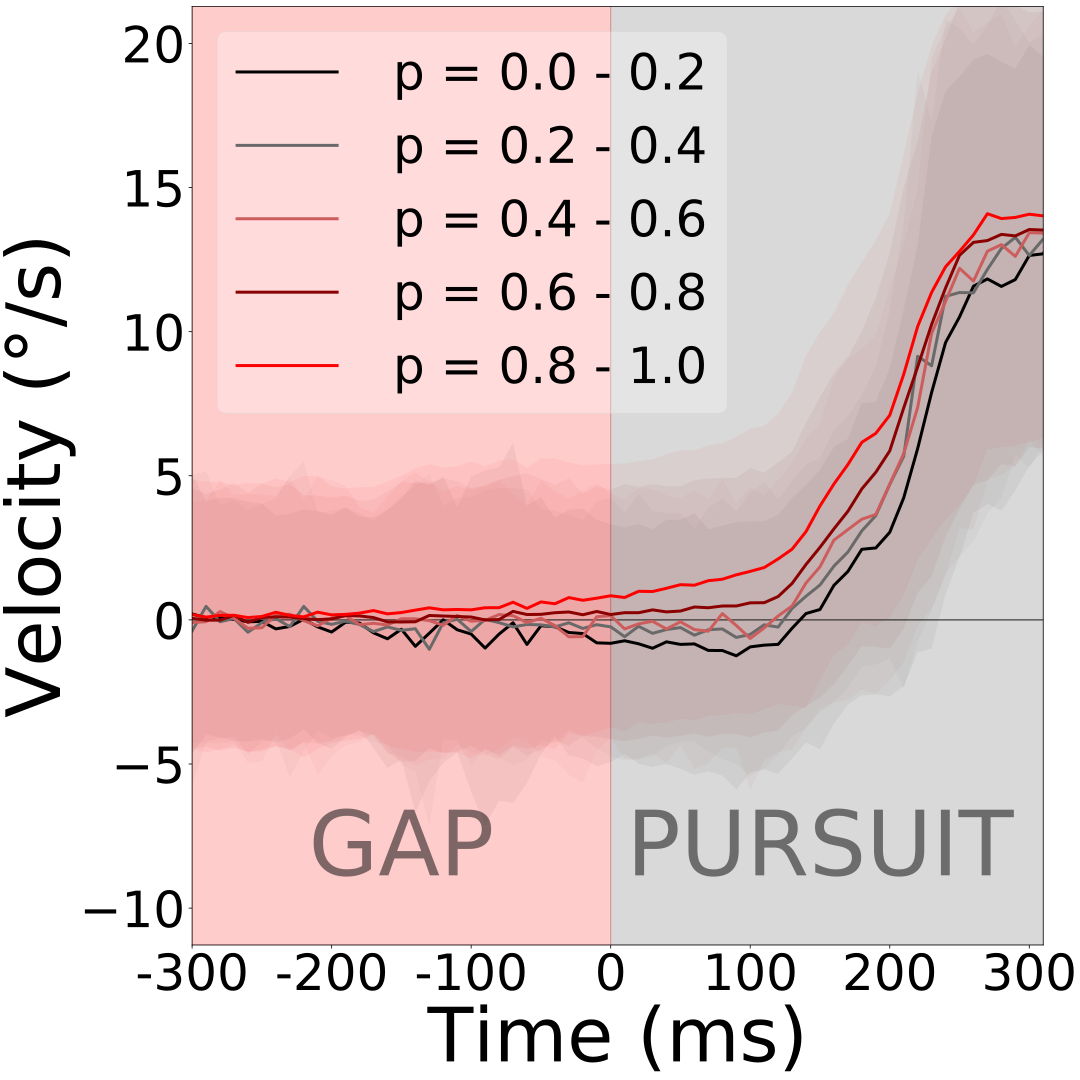
\includegraphics[width=0.33\linewidth]{1_B_Trace_moyenne}};
%\node [anchor=north west]  (img2) at (0.5\linewidth,.618\linewidth){\includegraphics[width=0.25\linewidth]{image_anna_1}};
% cf 0_protocole.ipynb
\node [anchor=north west]  (img2) at (0.844\linewidth,.538\linewidth){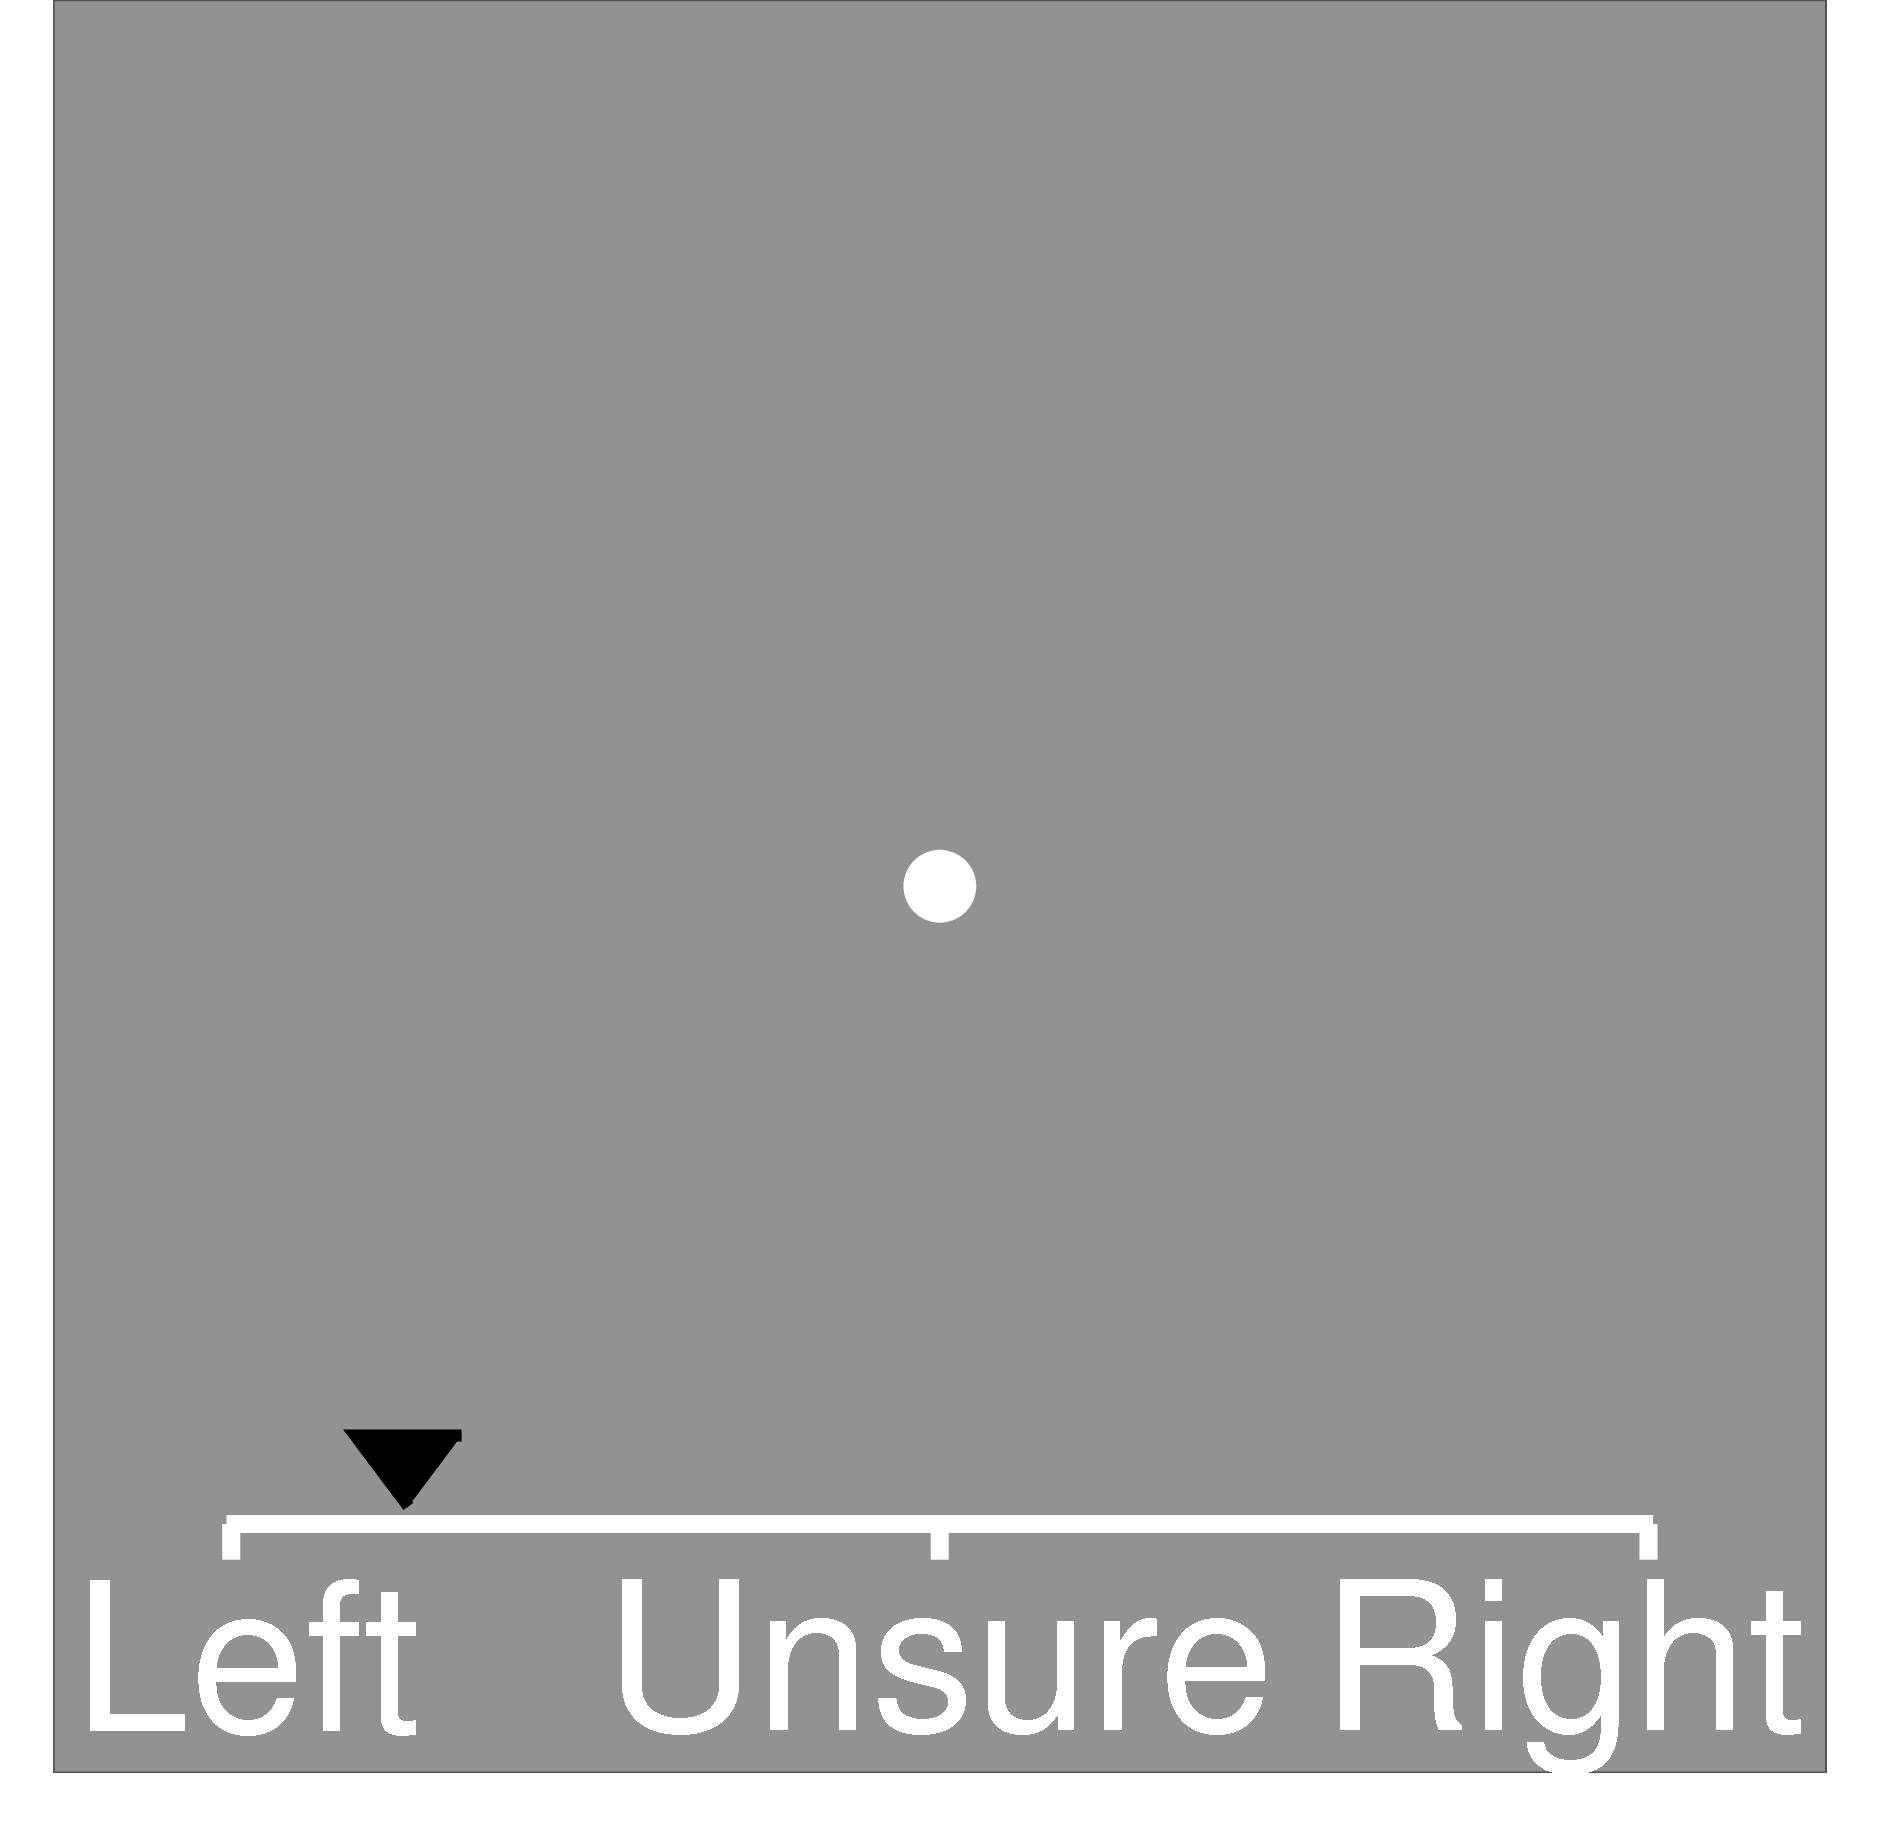
\includegraphics[width=0.156\linewidth]{1_C_protocol_bet_simple}};

%\node [anchor=north west]  (img2) at (0.75\linewidth,.618\linewidth){\includegraphics[width=0.25\linewidth]{protocol_bet_simple}};
\draw [anchor=north west] (0.000\linewidth, .62\linewidth) node {$\mathsf{(A)}$};
\draw [anchor=north west] (0.505\linewidth, .62\linewidth) node {$\mathsf{(B)}$};
\draw [anchor=north west] (0.842\linewidth, .62\linewidth) node {$\mathsf{(C)}$};
\end{tikzpicture}

\caption{\emph{Anticipatory SPEM (aSPEM): experimental design and results. \textbf{(A)}~# TODO: MOVE THIS PART IN THE MAIN TEXT}:
We replicated the results of~\citet{Montagnini2010},
in which human observers were presented with several $500$ trials blocks of horizontal target motion with a block-dependent direction probability bias, and they were asked to track the target with their gaze.} % TODO:check
The eye-movements task was an atapted version of a task developed by ~\citet{Montagnini2010}. Each one of $600$ trials consisted of sequentially:
a fixation dot (of random duration between $400$ and $600$~\ms),
a blank screen (of fixed duration of  $300$~\ms) and
a moving dot (at \AM{TODO CHECK! $10$ deg/s}) which the observers were instructed to follow.
The direction of the dot was drawn pseudo-randomly
according to a binomial distribution
parameterized by a probabilistic bias $p$
($0\leq p\leq 1 $). The direction is unbiased for $p=0.5$,
always left for $p=0$ and always right if $p=1$.
\AM{I DON'T THINK THAT WE HAVE DONE THIS EXPERIMENT! In a first experiment,
we %replicated the experiment of~\citep{Montagnini2010} and
tested $5$ different values of $p$:
$.25$, $.5$, $.75$, $.9$ and $1.$,
in fixed blocks of $120$ trials each.}
% TODO : dans notre plot on a des range de valeurs pour p :-/ -> C'EST PARCE QUE LE PLOT REPRESENTE DEJA LA VITESSE MOYENNE OBTENUE DANS LA TACHE AVEC SWITCHES!
\textbf{(B)}~Velocity traces of eye movements
averaged, over observers, for five different intervals of the direction bias.
These traces are aligned to the onset of the moving dot.
Saccades were removed using a thresholding method~(see \seeApp{em}) and
error bars show one standard deviation over all samples.
In the unbiased condition, one can distinguish
a visually-driven component (after a latency of $\approx 100~\ms$)
which corresponds to a standard Smooth Pursuit Eye Movement (SPEM).
When introducing a bias in the direction,
one observes that the average velocity of the eye progressively ramps
in the direction of the expected velocity, starting during the GAP phase and well before the visually-driven component:
This phase is the Anticipatory SPEM (aSPEM).
As reported previously~\citep{Montagnini2010, SantosKowler2017,Damasse18},
the slope of this ramp correlates with the strength of the bias.
%\LP{say this in words or in the ANnex: "This is shown in the inset showing the average gain in velocity ($\pm$ SEM)
%before any visually driven information (here, at $t=50~\ms$)." or refer to the recent publication from JB}
\textbf{(C)}~In this paper, we extended this experiment in three aspects.
First, we used probability biases in a continuous space,
as drawn from a prior distribution for the values of $p$.
Second, \AM{we generated the random sequence of trials
by concatenating random-length blocks (see \seeFig{results_raw}),
to avoid potential confounds related to the previously used blocked-design}.
Third, in order to titrate the adaptation to the environmental volatility at the conscious level,
we invited each observer to perform a variant of the direction-biased experiment on a subsequent day,
where, instead of recording their eye movements, we asked participants to rate the level of confidence
for their estimate of the forthcoming direction of the dot before each trial.
As shown in this sample screenshot,
this was performed by moving a mouse cursor on a rating scale
between ``sure left'', to ``unsure'' and finally ``sure right''.
%Eye movements were not recorded.
%Due to the (pseudo-)random nature of the sequence no observer noticed
%that the same sequence of directions was used in the experiment.
}
\label{fig:intro}
}
\end{figure}

%-------------------------------------------------------------%
%: adaptation to volatility in EMs : seen as an anticipation in SPEM - principle and function
Humans are able to accurately track a moving object
with a combination of saccades and
Smooth Pursuit Eye Movements (SPEM)~\citep{ref}.
These movements allow us to align and
stabilize the object on the fovea,
thus enabling high-resolution visual detection.
This process is retarded by different factors such as axonal transduction,
neural processing and the inertia of the oculomotor system~\citep{Krauzlis89}.
When predictive information is available about target motion,
anticipatory SPEM (aSPEM) are
efficiently generated before target's appearance~\citep{Westheimer1954, Kowler1979a, Kowler1979b} thereby reducing visuomotor latency.
Moreover, some experiments have demonstrated the existence
of prediction-based smooth pursuit during
the transient disappearance of a moving target~\citep{Badler2006,BeckerFuchs1985}.
Overall, although the initiation of SPEM is almost always driven by a visual motion signal, it is now clear that smooth pursuit behavior
can be modulated by extra-retinal, predictive information even in the absence of a direct visual stimulation.
The anticipatory smooth pursuit behavior is remarkable
in different aspects.
First, its buildup is relatively fast, such that only a few trials are sufficient
to pick up some regularity in a binary sequence of alternating Right-Left directions.
Second, it is in general an unconscious process
of which participants are not aware of.
As such, this behavior is a \AM{potentially a useful marker
to study the internal representation of motion expectancy (or Prior) and in particular to analyze} how sensorimotor expectancy interacts dynamically with contextual contingencies in shaping (oculomotor) behavior.

%: linear relationship (talk about santos & kowler and others)
Typically, aSPEM is observed after a temporal cue and
ahead of target motion onset~\citep{Kowler1979a,Kowler1979b, Kowler1984}. %~(see \seeFig{intro}-A).
It is generally assumed that the role of anticipatory eye movements is
to minimize as fast as possible the visual impairment due
to the amplitude of eye-to-target position and velocity mismatch.
\AM{I WOULD POSTPONE THIS SENTENCE SOMEWHERE ELSE, AS IT IS DISTRACTING HERE... The compromise between speed and accuracy is shaped
by the variability introduced by the neural noise
at the neuro-motor junction~\citep{Harris98}.}
Overall, this reduces the typical sensorimotor delay
between target motion onset and foveation~\citep{REFNEEDED}.
In a previous study~\citep{Montagnini2010},
we have analyzed how forthcoming motion properties,
such as target speed or direction, can be
predicted and anticipated with coherently oriented eye movements~(see \seeFig{intro}-A).
It has been observed that the strength of anticipation,
as measured by the mean anticipatory eye velocity,
increases when the target repeatedly moves in the same direction~\citep{Kowler1984, Kowler1989, Heinen2005}.
We similarly found a graded effect of both the speed and the direction-bias
on the strength of aSPEM (see \seeFig{intro}-B).
In particular, this effect is linearly related
to the probability of motion's speed or direction~(see \seeFig{intro}-B).
These results are coherent within previous oculomotor findings
by our and also other groups~\citep{SantosKowler2017}.
These results imply that the probability bias over a target's direction is
one additional factor beyond other physical and cognitive cues~\citep{Kowler2014, SantosKowler2017,Damasse18}
that modulate the common predictive framework
driving anticipatory behavior to optimize a rapid and
precise foveation of the target on its expected future path.

%: limits of the previous method
In order to generalize such results to more ecological conditions,
it is necessary to extend the experimental protocol of~\citet{Montagnini2010} in three aspects.
First, it seems important to investigate the integration of environmental statistical regularities
in this smooth tracking task with
a large family of direction-biases for the target motion.
As such, instead of a finite set of probability biases, % ($.25$, $.5$, $.75$, $.9$ and $1.$, see \seeFig{intro}-B),
we decided to use a continuous range of probability biases~$p$.
%which we were sampling from a fixed prior distribution.
Second,~\citet{Maus2015} have recently shown that
both perceptual adaptation for speed estimation
and priming of aSPEM could occur simultaneously.
They found a robust repulsive adaptation effect
with perceptual judgements biased in favor of faster percepts
after seeing stimuli that were slower and~\textit{vice-versa}. \AM{Concurrently, these authors also found
a positive effect on anticipatory smooth pursuit, with faster anticipation after faster stimuli.}
Indeed, both priming and adaptation can hypothetically share
a common internal representation of stimulus' speed,
reasonably built according to the mean velocity of the last observed movements.
The comparison of the internal representation of speed
with the current stimulus velocity could explain repulsive aftereffects and,
at the same time, be used to elicit
an aSPEM component at the appropriate velocity
for next stimulus occurrences.
\citet{Maus2015} estimated the past history effects over different times scales,
with the priming effects being maximized
for short stimulus histories (around $2$ trials) and
adaptation for longer stimulus history, around $15$ trials.
Their main conclusion was that
perceptual adaptation and oculomotor priming
are the result of two distinct readout computational processes using the same internal representation of motion regularities.
Both these history lengths can be considered
short in comparison to the several hundreds
of trials that are commonly used in psychophysics and sensorimotor adaptation studies.
% ------------------------------------------------------------------
\subsection{Contributions}%Outline}
% SUMMARY : what is novel in our work
% ------------------------------------------------------------------
%: how we do it : or rather why we do it this way (and not like Matthys)
The goal of this study is to generalize the adaptive process
observed in the aSPEM response to more ecological settings but
also to broaden its scope by showing that such unconscious process
also occurs at the conscious level.
To analyse the effect of history length in all generality,
we therefore extended the protocol such that the probability bias
is fixed in sub-blocks with variable block lengths.
%The equations for this protocol will be detailed below~(\seeSec{bayesian_change_point}).
Indeed, by manipulating the probability for target motion direction,
as measured during a fixed duration gap
before target ramp-motion onset~(see \seeFig{intro}-A),
it is possible to bias the direction and mean velocity of aSPEM~(see \seeFig{intro}-B).
This suggests that probabilistic information may be used
to inform the internal representation of motion prediction
for the initiation of anticipatory movements~\citep{Montagnini2010}.
However, it is yet unclear what method to use
to dynamically manipulate the probability of the input sequence.

First, one possible confound in the previous study
is that the range of possible biases is finite and
that there is no direct experimental evidence that
any continuous value within the possible range (that is, the segment $[ 0, 1 ]$)
may be picked up by the visual system.
Second, another possible caveat comes from the fact that the sequence of blocks of conditions on $p$
was used within blocks of fixed lengths.
Indeed, observers may potentially pick up
the information on this fixed length
to predict the occurrence of switches in conditions.

Additionally, we observed qualitatively that following the switch from
one condition to the next,
the strength of aSPEM changed gradually,
consistently with other adaptation paradigms~\citep{Fukushima1996,Kahlon1996,Souto13},
but for which the adaptation mechanism was only fitted.
As a consequence, such estimate may become particularly
challenging in a dynamic context,
where the probabilistic contingencies vary in time in an unpredictable way.
In addition, whether and how the information processing underlying
the buildup of aSPEM and its dynamics is linked to
an explicit estimate of probabilities is unknown.
To alleviate this problem, we developed a new paradigm
in order to address this question
by explicitly modeling a dynamic process with a given volatility:
In particular, our design will make sure that one can manipulate the variable $p$
as a function of trial number by making $p$ itself a random variable. %,
% but also that we can devise an ideal observer for each sequence of inputs.
% TODO check transition
In order to understand the nature of the representation of motion regularities underlying eye movement adaptive behavior, it is crucial to collect verbal explicit judgments about expectations on motion direction, in addition to the recording of eye movements.
In such an explicit judgment task, we evaluated for each participant their confidence for the next trial direction
(\emph{prior} to the appearance of the target).
%on a rating scale
%between "sure left", to "unsure" and finally "sure right"~(see \seeFig{intro}-C).


%\subsection{Generative model: the binomial switching model}
%-------------------------------------------------------------%
%: FIGURE 2 fig:results_raw ~\seeFig{results_raw}
% cf 1_generative-model.ipynb
\begin{figure}%[b!]
\centering{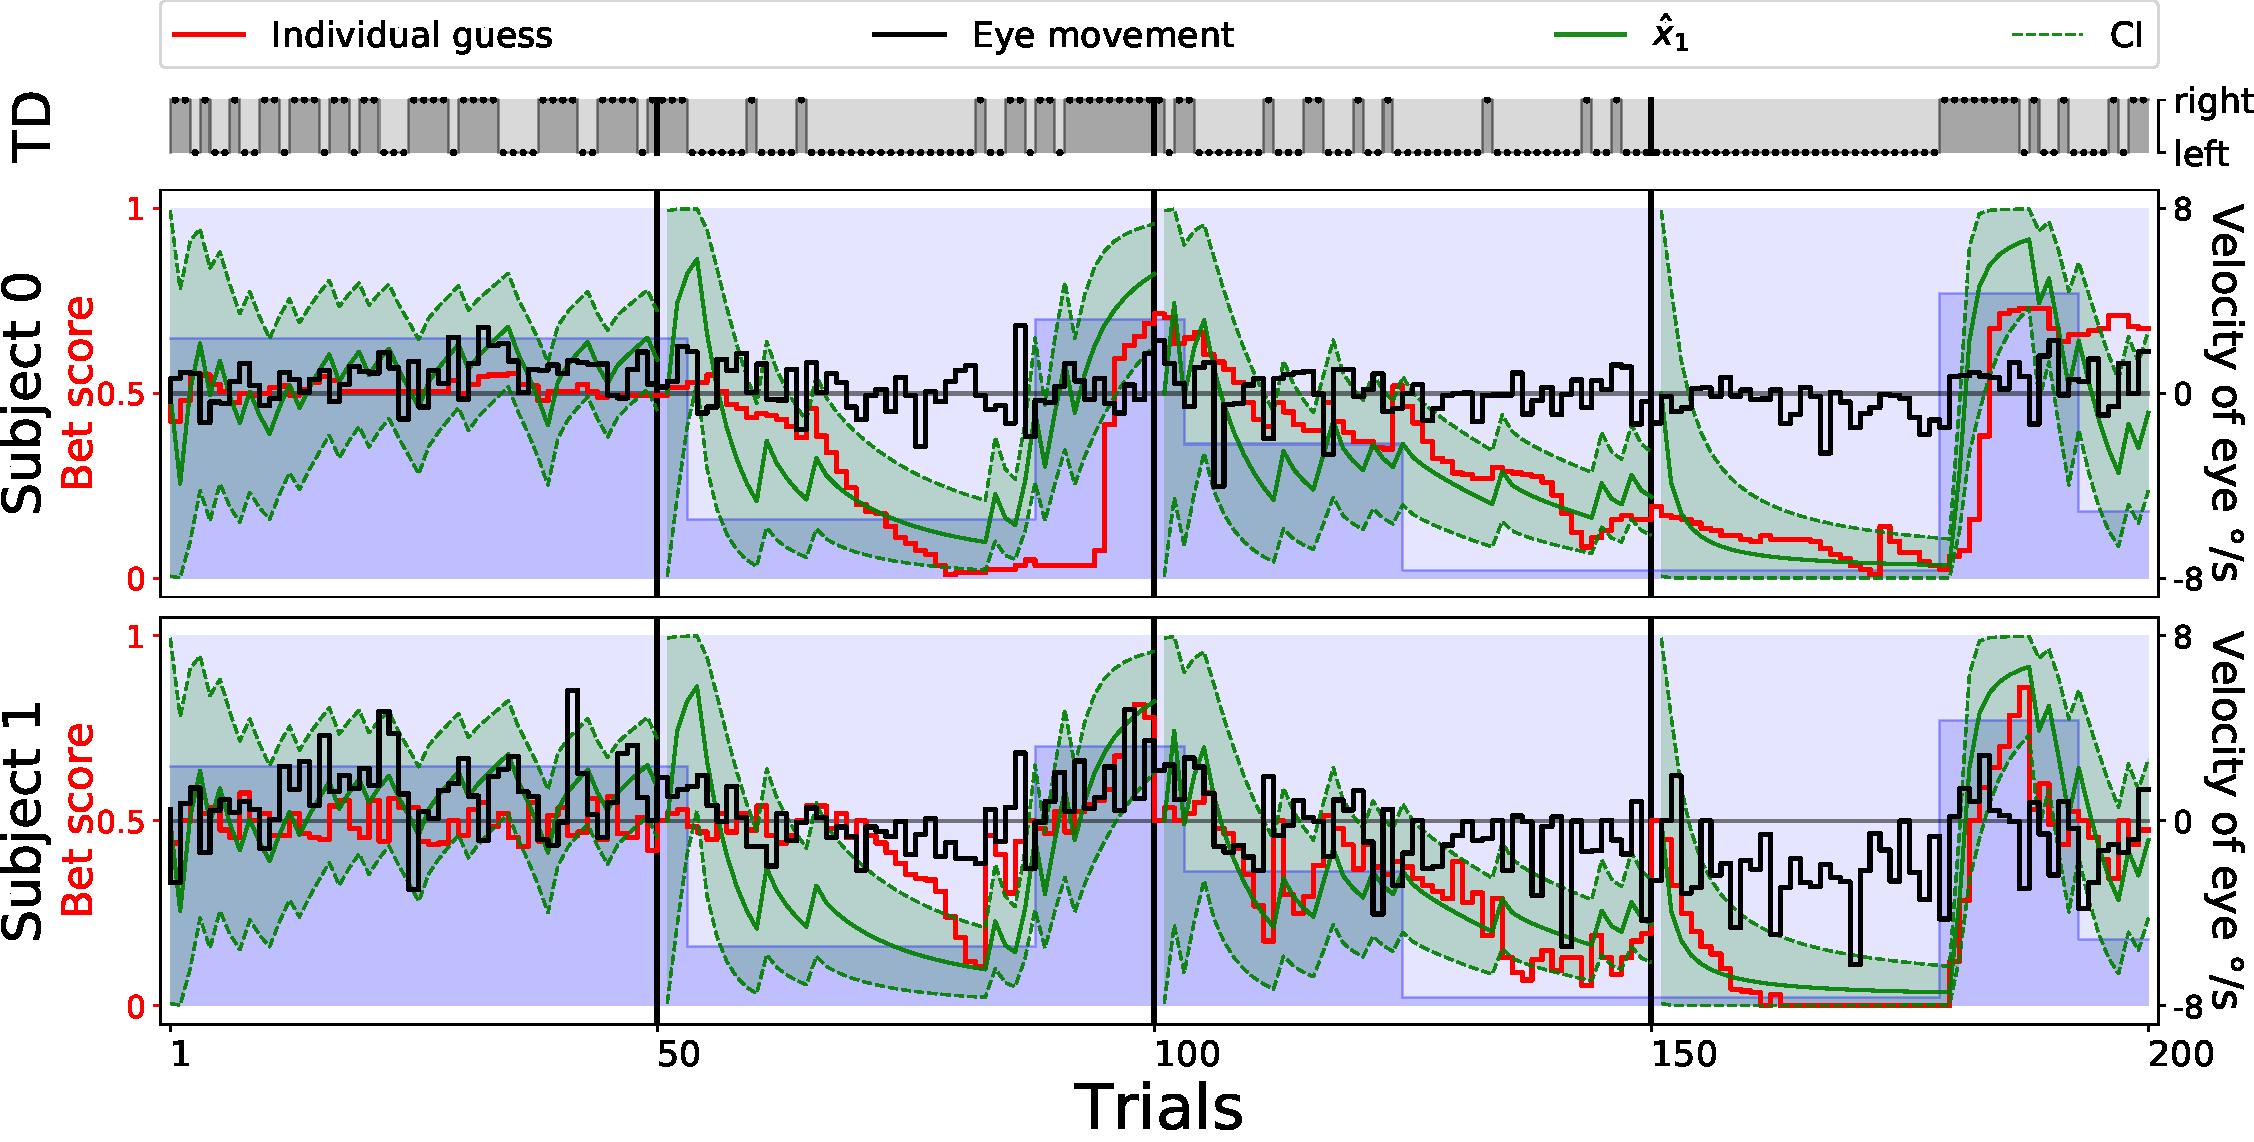
\includegraphics[width=\linewidth]{2_results_enregistrement}}
\caption{
\emph{The binomial switching model and raw psychophysical results.}%
~\textbf{(A)}
This diagram represents an instance of a sequence of directions (one ``block'')
as generated by the binomial switching model. %
%It is represented as a graphical model representing
%the three levels of the stochastic model. %
\LP{"TD" > "BSM" + make A bigger compared to B}
We plot
1/ the (hidden) evolution of the value of $p$ (horizontal blue areas)
and the underlying times for switches (vertical black lines : TODO).
\LP{legende pour la trace bleue}
2/ the sequence of target directions
and that were presented to observers
(red or black dots for respectively left or right directions :TODO).
It is a binary random variable which varies dynamically
as a function of the number of trials.
Each participant see 3 blocks of $200$ trials,
once for eye recording~(see \seeFig{intro}-A)
and in a subsequent day for the rating scale experiment~(see \seeFig{intro}-C).
Note that we introduced pauses every $50$ trials to prevent from fatigue.
~\textbf{(B)} Raw results for two characteristic observers.
% Each block is divided in 4 sub-blocks of $50$ trials as denoted by vertical black bars
Using a pseudo-random number generator with the same seed,
we could present the exact same sequence to all subjects. %
We have superposed the trace of
1/ as above (hidden) dynamics of $p$ and switches (vertical black lines : TODO).
2/ the recorded aSPEM strength as measured by the horizontal displacement
at the onset of the visually-driven SPEM (black line);
these values were here scaled according to their extremal values,
and we show as an horizontal dashed line the zero value.
3/ the response to the rating scale experiment (red line) and
%3/ the result of the BBCP model (blue line)
%along with the confidence interval for this estimate (blue shaded area).
\LP{"Bet of probability" > "Value of bet"}
Qualitatively, there seems to be a trend with the polarity of aSPEM
to be negative for $p$ values below~$.5$ and positive for values above~$.5$,
but also that the consciously predicted value
for the next outcome
seem to follow a similar trend.
}
\label{fig:results_raw}
\end{figure}
%-------------------------------------------------------------%
%: design of the binomial switching generative model
Indeed, to assess the dynamics of the adaptive processes
which compensate for the variability of sensory sequences,
one may generate random sequences for the value of $p$,
with a parametric mechanism controlling for the volatility at each trial.
By definition, volatility measures the temporal variability
of the sufficient parameters of a random variable.
% \AM{THEN I HAVE A QUESTION: GIVEN THIS DEFINITION, DOES VOLATILITY CHANGE AT EACH TRIAL IN OUR CASE, OR IS VOLATILITY FIXED ONCE THE TAU=40 PARAMETER HAS BEEN CHOSEN?} it is given by tau /on average/
In the \emph{Hierarchical Gaussian Filter} model (HGF, ~\citet{Mathys11}) for instance,
volatility is controlled as a non-linear transformation
of a random walk (modeled itself by a Brownian motion with a given diffusion factor).
This hierarchical model allows to ultimately generate a sequence of binary choices
where the variability fluctuates along a given trajectory.
Such a forward probabilistic model is invertible
using some simplifying assumptions and allows
to extract an inference of the agent's belief about volatility~\citep{Vossel14}.
Herein, we will use a simpler model where
the bias $p$ in target direction varies according to a piecewise-constant function
%(that is, a step function varying between~$0$ and~$1$),
similarly to~\citet{Meyniel13}.
Indeed, within each sub-block, the volatility of the value of $p$
progressively decreases as we accumulate samples.
It means that instead of a complex stochastic trajectory,
we draw random events (that we denote as ``switches'')
with a given mean frequency,
and that the bias in target direction is stationary between two switches:
The value $p$ of the bias only changes at the moment of a switch,
independently of the previous bias' value.
Such a sequence is presented in~\seeFig{results_raw}-A, %TODO : add A + blue line
where we show the realization of the target's directions sequence (above), and
below the trajectory of the underlying (hidden) $p$ bias' probability.

% equations
Mathematically, this can also be considered as a three-layered hierarchical model
defining the evolution of the model for each trial $t$ as the vector  $(x_2^t, x_1^t, x_0^t)$.
At the topmost layer,
the occurrence $x_2^t \in \{ 0, 1 \}$ of a switch ($1$ for true, $0$ for false)
is  drawn from a Bernoulli process with the switch's frequency $1/\tau$ as the main parameter.
The value of $\tau$ thus gives the average length (in number of trials)
between the occurrence of two switches.
The probability bias $p$ in target direction is a random variable that we define as $x_1^t \in [0, 1]$.
It is chosen at random from a prior distribution $\Pp$ at the moment of a switch,
and else it is constant until the next occurrence of a switch.
Finally, a target moves either to the left or to the right,
and we denote this variable (target direction) as $x_0^t \in \{ 0, 1 \}$.
This direction is drawn from a Bernoulli process $\Bb$
parameterized by the direction bias $p=x_1^t$.
Mathematically, this is easily described
by a 3-layered graphical model according to %~(\seeFig{results_psycho}-A) and
the following equations:
\begin{itemize}
    \item Occurrence of a switch: $x_2^t \propto \Bb(1/\tau)$
    \item Dynamics of probabilistic bias: \eql{\choice{\text{if} \quad x_2^t=0 \quad \text{then} \quad  x_1^t = x_1^{t-1} \\
\text{else} \quad x_1^t \propto \Pp  }\label{eq:bsm}}
    \item Sequence of directions:  $x_0^t \propto \Bb(x_1^t)$
\end{itemize}
% \eql{\choice{
% x_2^t \propto \Bb(1/\tau) \\
% % TODO: nest the choice
% \choice{\text{if} \quad x_2^t=0 \quad \text{then} \quad  x_1^t = x_1^{t-1} \\
% \text{else} \quad x_1^t \propto \Pp  \\
% } \\
% x_0^t \propto \Bb(x_1^t)
% }\label{eq:bsm}}
Note that the prior distribution $\Pp$ can be for instance
the uniform distribution $\Uu$ on $ [ 0, 1 ] $ or
Jeffrey's prior $\Jj$~(see \seeApp{bcp}).
There is always a switch at $t=0$ (that is, $x_2^0=1$). % and optionnally for each pause \AM{Is this true?} no it wasn't.
Herein, the experimental protocol is similar
to that presented in~\seeFig{intro}-A,
except for the pseudo-random sequence of directions $x_0^t$.
This randomizes the occurrence of the switches,
the length of sub-blocks
and the continuous range of bias' values that are explored.
To sum up, The system of three equations~\seeEq{bsm}
defines the Binomial Switching Model (BSM)
which we will use for the generation of sequences in experiments
but also as the basis of an ideal observer model.

%: outline
This paper is organized in five parts.
After this introduction where we presented the motivation for this study,
the next section~(\seeSec{bayesian_change_point}) will present
an inversion of the BSM forward probabilistic model,
coined the Binomial Bayesian Change Point (BBCP) model.
To our knowledge, such algorithm is not available yet, and
we will here provide it with an analytical solution,
by extending previous results from~\citet{AdamsMackay2007}
to the case of binomial data as in the BSM presented above.
In addition, this solution is \emph{online},
that is, that all computations on the sequence may be done
using solely the variables available at the present trial,
compactly representing all history see in previous trials.
We will also provide a computational implementation
and a quantitative evaluation of this algorithm.
Then, in~\seeSec{eye_rec} we will present  the analysis of anticipatory eye movements
to validate the generalization of previous results %.
%In a first session, participants observe a target moving horizontally
%with constant speed from the center
%either to the right or left across trials
with this novel protocol. %~(see \seeFig{intro}-A \& B).
Such results will allow us to fit the inverse model and to compare
its prediction compared to classical models such as the leaky integrator model.
%The probability of either motion direction changes randomly in time.
In a second experimental session, participants were asked to estimate
``how much they are confident that
the target will move to the right or left in the next trial'' and
to adjust the cursor's position on the screen accordingly~(see \seeFig{intro}-C).
The results will be presented in~\seeSec{rating_scale}
and compared to the results for eye movements.
Similarly, we will show that these results fit well
with the inverse model.
In~\seeSec{inter}, we will synthesize these results
by inferring the volatility parameters extracted
for each individual participant. % and session.
This will allow the analysis of inter-individual behavioral responses for each session
and in particular if one could predict observers' prior volatility,
that is, a measure of the dynamic compromise between exploration (``should I stay?'')
and exploitation (``should I go?'')
across the two different sessions testing predictive adaptive processes
at the unconscious and conscious levels.
Finally, we will summarize and conclude this study and
offer some perspectives for future work in~\seeSec{outro}.
%: %%%%%%%%%%%%%%%%%%%%%%%%%%%%%%%%%%%%%%%%%%%%%%%%%%%%%%%%%%%%%%%
\section{Results: Binomial Bayesian Change Point (BBCP) model}
%%%%%%%%%%%%%%%%%%%%%%%%%%%%%%%%%%%%%%%%%%%%%%%%%%%%%%%%%%%%%%%%
%%%%%%%%%%%%%%%%%%%%%%%%%%%%%%%%%%%%%%%%%%%%%%%%%%%%%%%%%%%%%%%%
\label{sec:bayesian_change_point}
%%%%%%%%%%%%%%%%%%%%%%%%%%%%%%%%%%%%%%%%%%%%%%%%%%%%%%%%%%%%%%%%
%
%: short intro
%
As we saw above, Bayesian methods provide with
a powerful framework for studying human behavior.
In the HGF model~\citep{Mathys11}, for instance,
authors defined a multi-layered generative model for
sequences of input stimuli.
By ``inverting'' this stochastic forward process,
one could extract relevant descriptors at the different levels of the model
and fit these parameters with the recorded behavior.
Here, we will use a similar approach but on a different generative model,
as defined in~\seeEq{bsm}.
First, as a control, we will define a first ideal observer
which assumes that volatility is stationary with a fixed frequency.
Then, we will extend it by modeling an agent
which assumes that the value of the probabilistic bias changes only
at specific (yet randomly drawn) trials (switches),
as was modeled by the forward probabilistic model defined in~\seeEq{bsm}.
%
% ------------------------------------------------------------------
\subsection{Forgetful-agent model (Leaky integrator)}%
% ------------------------------------------------------------------
%: justification from previous studies
Following~\citet{Maus2015},
we modeled a first ideal observer,
which represents a widespread
realistic model of how trial-history shapes
adaptive processes in human behavior,
for instance motion expectation in a direction-biased experiment.
First, according to~\citet{Anderson2006},
the temporal evolution of the expectation $p=x_1^t$ of a given event
can be modeled by making a simple heuristic:
the update of the estimated probability for an event is based
on the discount of the previously estimated probability
by a factor $1 - h \in [0, 1]$, relative to new information.
At trial $t$, this model can be expressed with the following equation:
%TODO fix the notation \hat{p}^{t+1} > \hat{p}(t+1)
\eql{%\choice{
% p^t = 0 \quad \text{if} \quad x_2^t=0 \\
\hat{x_1}^{t} = (1 - h) \cdot \hat{x_1}^{t-1} + h \cdot x_0^t
% }
\label{eq:leaky}}
where $\hat{x_1}^{t=0}$ is equal to some prior value ($.5$ in the unbiased case).
% NOTE: it's an AR(1) process https://stats.stackexchange.com/questions/358162/writing-ar1-as-a-ma-infty-process
%: from heuristics to ideal observer
The estimated  probability $\hat{x_1}^{t}$ results then from the integration of previous instances
with a progressive discount of past information.
The value of the scalar $h$ represents
a compromise between responding rapidly
to changes in the environment ($h \approx 1$) and
not prematurely discarding information still of value
for slowly changing contexts  ($h \approx 0$).
In the following, we will call this scalar the hazard rate.
Equivalently, one can define $\tau = 1 / h$ as
a characteristic time for the integration of information.
Looking more closely at this expression,
the ``forgetful agent'' computed in \seeEq{leaky}
consists in an exponentially-weighted moving average (see \seeApp{leaky}).
It is thus a form of moving average:
\eql{
\hat{x_1}^{t} = h \cdot \sum_{0\leq i \leq t} (1 - 1/\tau)^{i} \cdot x_0^{t-i}
\label{eq:leaky2}}
\AM{In principle there should also be a term proportional to $(1-h)^{t}$$\hat{x_1}^{t=0}$, true? Which tends to $0$ for large $t$...}
Inversely, let us assume that at each trial,
the true probability bias changes randomly with a rate of once
every $\tau$ trials.
As a consequence, the probability that the bias does not change is $Pr(x_2^t=0)=1-1/\tau$ at each trial.
Assuming independence of these occurrences, the estimated probability $p=\hat{x_1}^{t}$ is thus the sum
of the past observations weighted by the belief that the bias has not changed during $i$ trials in the past, that is exactly
as defined in~\seeEq{leaky2}.
This shows that ignoring the temporal occurrence of the switch,
the optimal solution to this problem is the
ideal observer defined in~\seeEq{leaky2},
which finds an online recursive solution in~\seeEq{leaky}.
% and which believes that changes occur at a constant rate ($\hat{x_2}^t=h$
We therefore proved here that the heuristic derived from~\citet{Anderson2006}
is an ideal inversion of the generative model
which assumes a fixed duration for the probability bias. %\AM{It seems to me that the main limit of this ideal observer is that it is lazy: it knows that on average things change every tau trials but it does nothing to actively estimate and account for these changes: maybe we should have a sentence here to introduce this concept of "active"/"adaptive" observer?} - LP : right, ours is indeed a more active agent, but that's quite subjective...

%: using \hat{p} as a regressor
The correspondence that we proved between the weighted moving average heuristic
and the ideal observer model as a solution to a generative model lead
us to several interim conclusions.
First, the time series of $\hat{x_1}^{t}$ values can serve as a regressor
to test whether human observers follow the same strategy.
In particular, one could test the parameter $\tau$, relative to the agents' belief in the weight decay:
importantly $\tau$ may be fitted to the data,
for instance to the data shown in~\seeFig{results_raw}.
However, one should be careful with such conclusions whenever
this trajectory is fitted to behavioral data.
For instance, if the inversion of the forward model is exact in the present case,
one has to use approximations in more complex models,
such as with the HGF~\citep{Mathys11} or the models developed by~\citet{Wilson13,Wilson18}
and some discrepancy could originate from these approximations
at the algorithmic level.
As such, it is essential that these both sources of discrepancy (intrinsic versus extrinsic)
should be controlled independently~\citep{Beck12}.
Second, if we assume that the inversion of the model is perfect
(that is, that no approximation has been done),
this means that by fitting different ideal observers
to the data, one evaluates as a matter of fact the adequacy of
a generative model, not to probabilistic calculus.
This is a common confusion around the idea of a ``Bayesian brain''.
We believe here that the challenge is not to validate the hypothesis that the brain uses or not the Bayes' theorem,
but rather to test different hypotheses about the generative models
that agents may use.
This may be essential in designing the experimental protocol,
or in evaluating quantitatively the results.

%: limits of the leaky integrator
Now, since we have defined a first generative model
and the ideal observer which it corresponds to,
we will define a more complex model
in order to overcome some of the limits of the leaky integrator.
Indeed, a first criticism could be that
this model may be too rigid and does not sufficiently
account for the dynamics of volatility~\citep{Behrens07}
or Bayesian uncertainty~\citep{Vilares2011}.
It seems plausible that the memory (history length) the brain uses
for inference is varying and that this variation could be related
to the volatility inferred from information in the past.
The model presented in~\seeEq{leaky2} uses a constant weight
(decaying with the distance to the current trial)
for all trials, while precision of each trial
can be potentially evaluated and used
for precision-weighted estimation of the probability bias.
To address this hypothesis, our next model work will be inspired
by a Bayesian Change-point detection model~\citep{AdamsMackay2007},
which models an ideal agent inferring
both the trajectory of the probability bias ($x_1^t$)
and the probability $Pr(x_2^t=1)$ of the occurrence of switches.
% ------------------------------------------------------------------
\subsection{Binomial Bayesian Change Point model}
% ------------------------------------------------------------------
%-------------------------------------------------------------%
%: >>>> LuP is here <<<<
%: FIGURE 3 fig:bayesianchangepoint \seeFig{bayesianchangepoint}
\begin{figure}%[b!]
% cf 3_Results_2.ipynb
\begin{center}
%\includegraphics[width=\linewidth]{figure3}
% cf : 3_Results_1
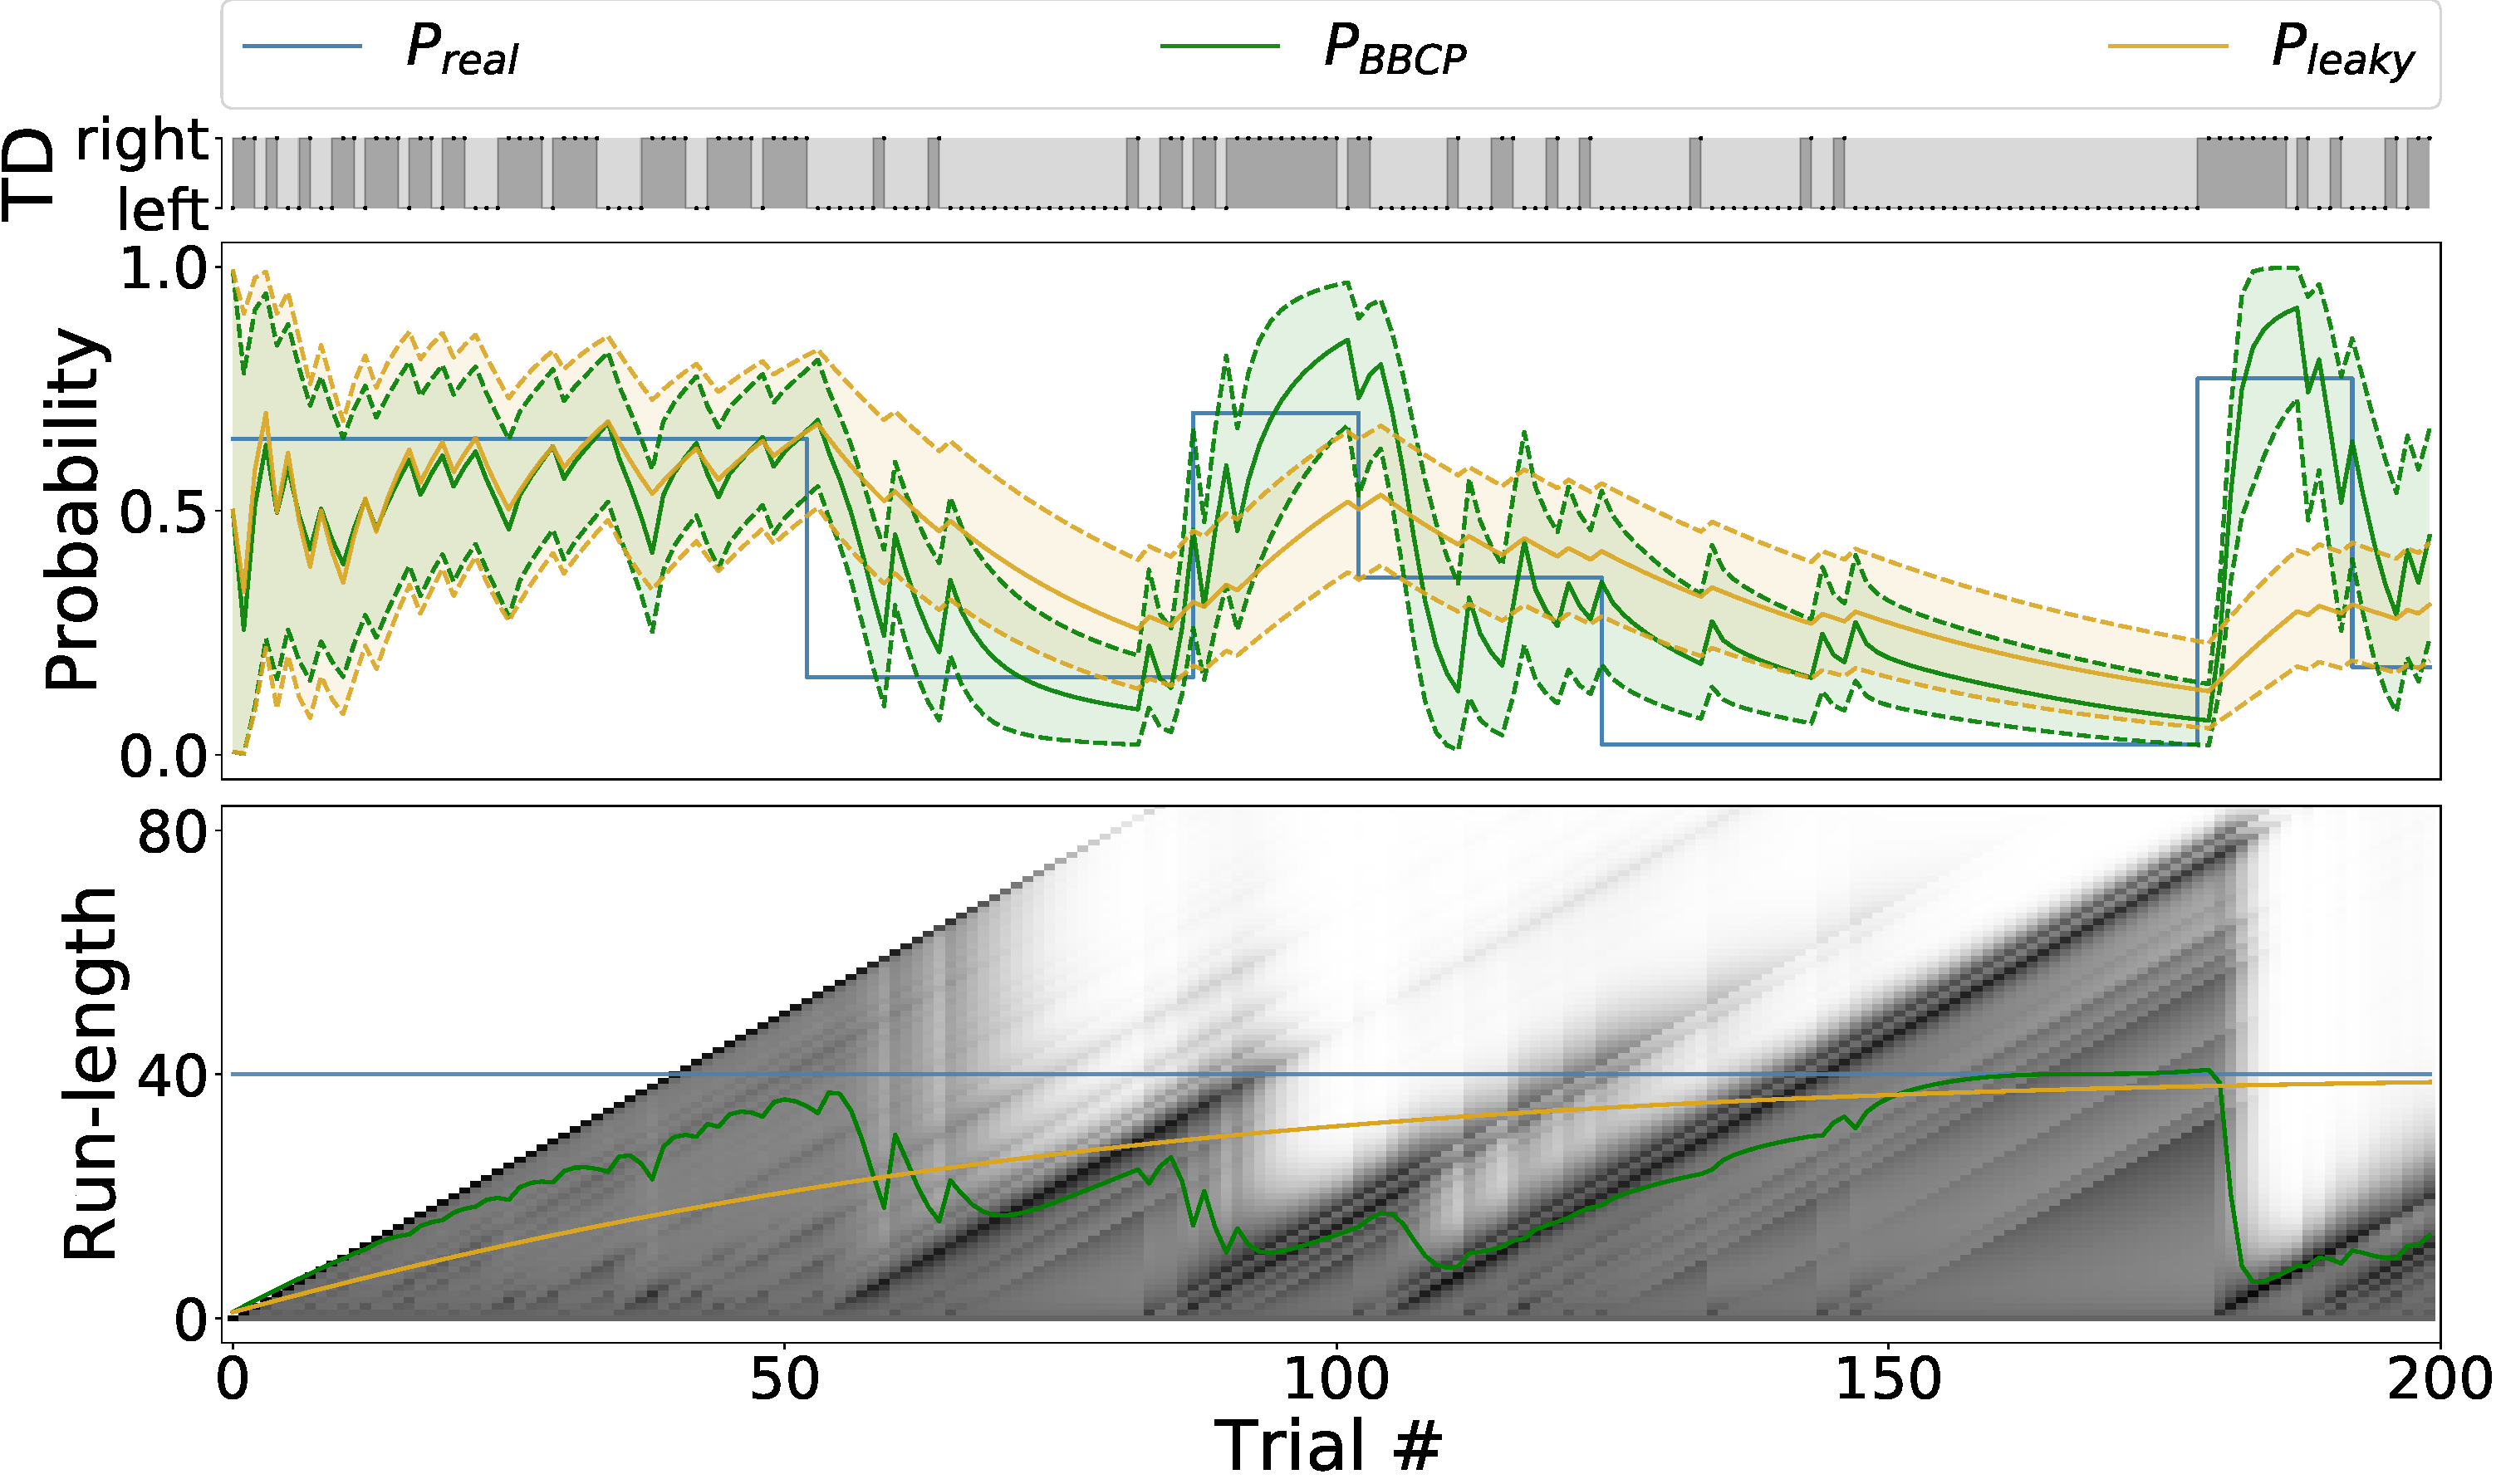
\includegraphics[width=1\linewidth]{3_BCP_readouts}
\end{center}
\caption{\emph{Binomial Bayesian Change Point model}
% (A) le principe de l'algorithme, \AM{Caption does not correspond to the figure!}
~\textbf{(A)} shows a synthesized sequence of events that works as a binomial choice, either $0$ or $1$.
In particular, the probability switched at trials 6 and 10.
We show the graph (treillis) on which the message indicates that
mass probability is being passed.
Black lines denotes ``upwards'',
that is, for which there is a progression of the run length at the next step.
The red line stands for the possibility that a switch happened,
and then falls back to zero.
The black curve stands for
the run length of simulated data in~\textbf{A}
as a function of time (r$_t$).
We can see that
the run length drops back to zero
when change occurs at trials 6 and 10.
%(B) le résultat sur une séquence et
~\textbf{(B)} is a sequence of points representing
leftward (0) of rightward trials (1)
with a given probability $p$ of being rightward and
that changes at some trials (clear red).
The predicted probability $\hat{p}$ ($\tau=N_{trial}/4$ tells the BBCP
that the probability is more susceptible to change every $1/h=N_{trial}/4$),
continue and dotted dark red lines shows the $p$$-$estimation.
\LP{ older stuff: ``We show two panels, one below which displays
the value of the belief for the different run-length,
and one above where we will show the resulting prediction of the next outcome.
We obtain for any given sequence different values at the given trial
in the form of columns for any possible run-length:
the belief, and the sufficient statistics for the beta distribution
which allow to provide with an estimate of the current probability.
First, we show the value of probability,
low probabilities are blueish while high probabilities.
At every trial, the agent evaluates the value
for the different possible run lengths, generating a column.
By showing all columns we generate this image
which shows the evaluation along the sequence of trials.
Second we show above the sequence of observations
that were shown to the agent in a light black line.
The red line gives an evaluation of the most probable
a posteriori probability as the probability to the run-length
the maximum a posteriori belief on the different beliefs about run-lengths. ''
%using the estimate of the precision at this
% (C) une analyse quantitative qui permettra de l'utiliser pour les expériences psycho
}
~\textbf{(B)} shows the probability of the run length,
the probability of the having same probability consecutive trials.
The red line represents the $\hat{r}$,
that represents the sum of he products of each r
(number of consecutive trials having the same probability)
$\sum_{r=0}^\infty r \cdot P(r)$.
~\textbf{C} represent the probability of each r for trials 50 and 250
along their $\hat{r}$ and their $\hat{p}$.
For instance, for trial 50, we can observe that $\hat{r}$ is close
from the real number of trials during the probability has not changed (real $p$ stayed for 50 trials).
$\hat{p}$ is also pretty close from the real $p$ ($p=1$).
~\textbf{D} shows that at trial 250 $\hat{r}$ is more far than the real r
that is also equal to 50 trials.
But here, $\hat{p}$ is closer from $p$ that is equal to 0.75.
}
\label{fig:bayesianchangepoint}
\end{figure}
%-------------------------------------------------------------%
%-------------------------------------------------------------%
%: 2Ba precision in our belief of \hat{p}
%-------------------------------------------------------------%
There is a crucial difference between the simple agent presented above
which believes that changes occur at a constant rate ($\hat{x_2}^t=h$, see~\seeEq{leaky2})
and one that would invert the binomial switching model (BSM, see~\seeEq{bsm}).
Indeed, at any trial during the experiment,
the agent may infer beliefs about the trajectory of the volatility $x_2^t$
which itself is driving the trajectory of the probability bias $x_1^t$.
Knowing that the latter is piece-wise constant,
an agent may therefore have a belief over the number of trials since the last switch.
This number, that we will call the \emph{run-length}, is useful in two manners.
First, it allows for the agent to restrict the estimation $\hat{x_1}^{t}$ of $x_1^t$
to only those samples $x_0^t$ produced since the last switch and until $t$.
Indeed, the samples $x_0^t$ occurred before the switch are drawn independently from the present true value $x_1^t$
and thus cannot help estimating the latter.
Second, it is known that for  this estimate, the precision
(that is, the inverse of its variance)
grows linearly with the number of samples:
The longer the run-length, the sharper the corresponding (probabilistic) belief.
%Knowing a distributed belief on each different possible run-lengths, %  about different hypothesis
%as represented by the probability distribution of each hypothesis,
%the agent may therefore give different weights to the information
%using an evaluation of the precision of each respective hypothesis.
We have designed such an agent by extending
the Bayesian Change-Point (BCP) detection model~\citep{AdamsMackay2007}.
This model defines the agent as an inversion of a switching generative model
for which the observed data (input) is Gaussian.
We will here present an exact solution for the case of the BSM,
that is, were the input is binomial (see~\seeEq{bsm}).

%-------------------------------------------------------------%
%: 2Bb overcoming this difficulty using a latent variable - prediction/update cycle
%-------------------------------------------------------------%
In order to define in all generality the switch detection model,
we will describe the fundamental steps of its computation,
while giving the full algorithmic details in~\seeApp{bcp}.
A fundamental procedure in Bayesian predictive models is to introduce
a latent variable which helps the agent to represent the input.
%By construction of the generative model,
%a relevant latent variable is here the run-length.
Knowing that the data is generated by the BSM (see~\seeEq{bsm}),
the run-length is either null at the moment of a switch,
or is incremented by $1$ if no switch occurred:
\eql{\choice{
r^t = 0 \quad \text{if} \quad x_2^t=1 \\
\text{and else} \quad r^t = r^{t-1} +1 }\label{eq:run_length}}%see~\seeEq{run_length}
This may be represented in a graph
in which information will be represented at the different nodes for each trial $t$ (see \seeFig{bayesianchangepoint}-A).
Using this latent variable, the goal of predictive processing % \AM{predictive coding here comes as a "hair in the soup": it needs some noble introduction...}
is to infer the probability $Pr(x_0^t | x_0^{0:t-1})$ of the next datum
knowing what has been observed and
the prior of the agent on the generation of the data.
Mathematically, we will define the run length $r^t$ distribution
at each trial $t$ to represent our belief
for all different hypotheses as $\beta^{(r)}_t=Pr(r^t | x_0^{0:t-1})$.
%At each node, this assigns a probability strength
This allows to compute the marginal predictive distribution:
\eqa{
%\hat{x_1}^{t} =
Pr(x_0^t | x_0^{0:t-1}) &= \sum_{r^{t}} Pr(x_0^t | r^{t}, x_0^{0:t-1}) \cdot  \beta^{(r)}_t \\
%Pr(x_0^t | x_0^{0:t-1}) &= \sum_{r^{t}} Pr(x_0^t | r^{t}, x_0^{0:t-1}) \cdot  Pr(r^{t} | x_0^{0:t-1})\\
%\text{with} \quad Pr(r^{t} | x_0^{0:t-1}) &\propto \sum_{r^{t-1}}  Pr(r^t | r^{t-1}) \cdot  Pr(x_0^t | r^{t-1}, x_0^{0:t-1}) \cdot  Pr(r^{t-1} | x_0^{0:t-2})
\text{with} \quad \beta^{(r)}_t &\propto \sum_{r^{t-1}}  Pr(r^t | r^{t-1}) \cdot  Pr(x_0^t | r^{t-1}, x_0^{0:t-1}) \cdot  \beta^{(r)}_{t-1}
\label{eq:pred}
}

% \AM{the expression seems ok but some words saying why we are decomposing beta in this way would help}
%to represent our belief at trial $t$
%or to determine the pdf for $x_1^t$ as a mixture of Beta distributions:
%\eqa{
%\hat{x_1}^{t} =  \sum_{r^{t}} Pr(x_1^t | r^{t}, x_0^{0:t}) \cdot Pr(r^{t} | x_0^{0:t})
%}

First, we will \emph{update} beliefs on all nodes %\AM{the terms nodes and graph -later- are not intuitive for everyone...maybe a Figure could help?} that's what we tried to include in the figure of the model
 % at trial $t$
by computing the likelihood of the new datum $x_0^t$ knowing the current belief at each node that we define as $\pi^{(r)}_t=Pr(x_0^t | r^{t-1}, x_0^{0:t-1})$.
Second, knowing this probability strength, % an estimate for our belief on the different variables at the previous trial $t-1$,
we can make a \emph{prediction} for our belief of the state at the current trial $t$,
prior to the observation of a new datum $x_0^{t+1}$.
In the graph, this corresponds to a message passing from the nodes at time $t-1$
to that at time $t$ and formalized by the transition matrix $Pr(r^t | r^{t-1})$.
Finally, this update / prediction cycle applied to the BSM and using~\seeEq{bsm}
will constitute the Binomial Bayesian Change Point (BBCP) detection model.

%-------------------------------------------------------------%
%: 2Bc online estimation: initialization
%-------------------------------------------------------------%
%Following the principle of Active Inference, % POMDP / active exploration of feature space
% it can be the mean and variance of a Gaussian, but in general it will be 2 parameters. in our case, we wish to estimate p (between zero and one) - it is characterized by the beta distribution (mathematically it is the conjugate of the bernouilli distribution)
%s of a beta distribution
The main difference between our algorithm and that of~\citep{AdamsMackay2007},
is that the observed data is binomial and not Gaussian as in their case.
The random variable $x_1^t$ is the probability bias used
to generate the sequence of events $x_0^t$ through a binomial trial.
Mathematically, a belief on the probability bias $p$ defining the binomial trial (and thus to the process corresponding to the trial sequence),
is well represented by the conjugate probability distribution of the binomial distribution,
that is, by the beta-distribution $B(p; \mu, \nu)$,
which is parameterized here by its sufficient statistics,
the mean $\mu$ and sample size $\nu$
(see~\seeApp{likelihood} for our choice of parameterization).
First, beliefs are set at $t=0$ to prior values before observing the first trial.
In terms of probabilities, this amounts to set :
\eqa{
& \beta^{(0)}_0=Pr(r^0=0)=1 \text{,}\quad \forall r^0>0 \text{, } \beta^{(r)}_0=Pr(r^0)=0 \quad \text{and} \\
& Pr(x_1^0 | r^0=0) \propto B(x_1^0; \mu_{prior}, \nu_{prior})
%& P(r_0)= S(r) \quad \text{,} \mu^{(r=0)}_0 = \mu_{prior}\quad \text{and} \quad \nu^{(r=0)}_0 = \nu_{prior}
}
where $\mu_{prior}$ and $\nu_{prior}$ represent the sufficient statistics
of the prior (Beta-distribution) probability density function (pdf) $\Pp$
for the probability bias
at the occurrence of a switch (here at node $r^0=0$).
By recurrence, one can show that at any trial $t$,
this pdf will always be a beta-distribution,
but with varying sufficient statistics.
In the following, we will define the probability distribution at each node $r^t$,
knowing the data observed from the first trial and before $t$ such that
%$Pr(x_1^t | r^t, x_0^{0:t-1}) ~ B(x_1^t; \mu^{(r)}_{t}, \nu^{(r)}_{t})$.
%\eql{
$
\pi^{(r)}_t = B( x_0^t |  \mu^{(r)}_{t}, \nu^{(r)}_{t})
$. %}

%-------------------------------------------------------------%
%: 2Bd update = Computing the likelihood
%-------------------------------------------------------------%
%By introducing the run-length as a latent variable of our ideal observer,
%this algorithm introduced by~\citep{AdamsMackay2007}
%allows to infer the instantaneous volatility of the input sequence.
%It is equivalent as putting in competition
%different leaky integrators in parallel,
%one for each value of $r$ and to evaluate the probability $Pr(r_t | x_0^{0:t})$ for each of these hypothesis.
%and the uncertainty associated to it.
%As such, the main difference is the way that the likelihood is computed.
%https://en.wikipedia.org/wiki/Likelihood_function
%https://stats.stackexchange.com/questions/2641/what-is-the-difference-between-likelihood-and-probability
% https://en.wikipedia.org/wiki/Rule_of_succession
In particular, as we sequentially observe new data,
we will first implement an update step that
computes the likelihood of this datum $x_0^t$ with respect to
the current beliefs at trial $t$ at each node $r$.
In all generality, to perform this computation for some data $o$,
we have computed the probability of each model
parameterized by the mean $p$ and the sample size $r$
for the two hypothesis $o=1$ or $o=0$.
This defines the likelihood
$\Ll(o | p, r) = \frac{1}{Z} Pr(o |p, r)$
with $Z$ such that $\Ll(p | o=1, r) + \Ll(p | o=1, r)=1$.
It measures the relative frequency of observing an occurrence of $o$ at trial $t$,
as the updated estimation of the probability bias of $\frac{p\cdot r + o}{r+1}$
knowing a sample size of $r+1$.
%$\pi_{0:t} = P(x |\mu^{(r)}_t,\nu^{(r)}_t)$
Following the formulation of the beta probability distribution, it follows:
\eql{% TODO: check formula
\Ll(o | p, r) = \frac{1}{Z} \cdot {(p\cdot r + o)}^{p\cdot r + o} \cdot {((1- p)\cdot r + 1- o)}^{(1- p)\cdot r + 1- o}
\label{eq:likelihood}
}
where
\eq{
Z = {(p\cdot r + 1)}^{p\cdot r + 1}  \cdot {((1- p)\cdot r )}^{(1- p)\cdot r }  +
    {(p\cdot r )}^{p\cdot r }  \cdot {((1- p)\cdot r + 1)}^{(1- p)\cdot r + 1}
}
The derivation of this function is detailed in~\seeApp{likelihood}.
%The full algorithm is summarized in~\seeApp{bcp}.

%-------------------------------------------------------------%
%: 2Bd online estimation: prediction
%-------------------------------------------------------------%
%This computation is detailed below (see \seeEq{likelihood}).
In the second step, one can perform prediction
using the graph defined in \seeFig{bayesianchangepoint}-A.
Now that we have the vector of likelihoods $\pi^{(r)}_t=\Ll(x_0^t |  \mu^{(r)}_{t}, \nu^{(r)}_{t})$,
one can update probabilities and perform the next prediction for trial $t+1$.
%On the one hand, we determine the run length distribution
%\eqa{
%\beta^{(r)}_t = Pr(r_t | x_0^{0:t-1}) = Pr(r_t, x_0^{0:t-1}) / \sum_{r_{t}}  Pr(r_t, x_0^{0:t-1})
%}
%Based on the belief that was accumulated at trial $t$ %(see \seeFig{bayesianchangepoint}-B),
The transition matrix % defined by the graph,
allows to compute growth probabilities : %, that is, the belief at the next trial before observing a new datum:
\eqa{
\beta^{(r+1)}_t = \frac{1}{B} \cdot \beta^{(r)}_{t-1} \cdot \pi^{(r)}_{t} \cdot (1-h)
}
(where $h$ is the scalar defining the hazard rate)
but also the change-point probabilities:
\eqa{
\beta^{(0)}_t  = \frac{1}{B} \cdot \sum_{r} \beta^{(r)}_{t-1} \cdot \pi^{(r)}_{t} \cdot h
}
with $B$ such that $\sum_{r} \beta^{(r)}_{t} = 1$.
% Note that at $\forall t$,  $\beta^{(0}_{t}= h $
On the other hand, we update the sufficient statistics to be used in the computation of the likelihood at the next trial following:
\eqa{
& \mu^{(0)}_{t+1} = \mu_{prior} \text{,} \quad \nu^{(0)}_{t+1} = \nu_{prior} \\
& \mu^{(r+1)}_{t+1} = r/(r+1) \cdot \mu^{(r)}_{t} + 1/(r+1) \cdot x_0^t \text{,} \quad \nu^{(r+1)}_{t+1} = \nu^{(r)}_{t} + 1
}
Note that $\mu^{(r+1)}_{t+1}$ is a moving average at trial $t$ on the $r$ last samples,
and $\forall r, t; \nu^{(r)}_{t}$ is the sample size corrected by the initial condition:
$\nu^{(r)}_{t} = r + \nu_{prior}$.
This updates for each node the sufficient statistics of the pdf at the current trial.
This finalizes the prediction step.

The agent may infer at each trial the belief
and use for instance the expected value or the maximum a posteriori as readouts.
More precisely, we define these two strategies as following:
Either by chosing
at each trial the run-length with maximal probability
and then assigning the predicted probability bias
as the probability bias for that run-length:
\eql{
\hat{x_1}^t = \mu^{(r^\ast)}_{t} \quad \text{with} \quad r^\ast = \argmax_r \beta^{(r)}_{t}
}
A second strategy consists in computing
at each trial the conditional mean of the probability bias
as the expected value over all run-lengths:
\eql{
\hat{x_1}^t = \sum_{r} \beta^{(r)}_{t} \cdot \mu^{(r)}_{t}
}
Contrary to the leaky integrator for which the inference $\hat{x_2}=h$ was fixed,
the BBCP model uses a dynamical model, but still with only one parameter.
As for the latter, this parameter~$h=\frac 1 \tau$ informs the BBCP model
that the probability bias  changes \emph{on average} every~$\tau$ trials.
As in \seeEq{leaky}, this defines the \emph{hazard rate}.
Note that the resulting operations are online, that is,
that only the belief at trial $t$ and the new datum $x_0^t$
are sufficient to predict all probabilities.
%at the next trial $t+1$: $Pr(r_t | x_0^{0:t})$, $\mu^{(r)}_{t+1}$ and $\nu^{(r)}_{t+1}$.
%projecting beliefs backwards and forward  : the algorithm is online et the price of memory
% ------------------------------------------------------------------
\subsection{Quantitative analysis of the Bayesian change point algorithm}
% ------------------------------------------------------------------
%-------------------------------------------------------------%
%: 2Ca python scripts : qualitative analysis
%-------------------------------------------------------------%
We have implemented this algorithm using a set of python scripts.
This algorithm is detailed in~\seeApp{bcp} and provides also some control script
to test the behavior of the algorithm with synthetic data.
Indeed, this allows to qualitatively and quantitatively asses
this ideal observer with a known ground truth before applying it
on the trial sequence that was used for the experiments and compare it to the human behavior (see~\seeFig{results_raw}).
%TODO : synchronize with FIGURE 3 fig:bayesianchangepoint
\seeFig{bayesianchangepoint}~\textbf{A} shows
one instance of a sequence of simulated data $x_0^t$
of leftward and rightward trials with a probability $x_1^t$
of being rightward with possible variations across time.
It also shows the predicted probability $\hat{x_1^t}$
as computed using the BBCP algorithm.
\seeFig{bayesianchangepoint}~\textbf{B} illustrates
the belief on the predicted probability $\hat{p}$ at a given trial.
On \seeFig{bayesianchangepoint}~\textbf{C},
we can see the belief on the run length estimation.
We see that as in the synthetic example above,
there is a correct detection of switch after a short delay of a few trials.
We remark two main observations.
First, beliefs grow at the beginning along a linear ridge,
as we begin our model by assuming there was a switch at trial $0$.
Then, we observe that after a switch (hidden to the model),
the belief is diffused more strongly until the relative probability
is less that that assigned to a lower run-length.
Second, we may use this information to read-out the most probable probability-bias and the confidence interval
as shown by the red dashed lines (respectively $.05$ and $.95$).
Note, the fixed-length is simply implemented
by an agent with a fixed run-length $r_t=\tau$ (see broken dashed line in \seeFig{bayesianchangepoint}~\textbf{B})
this allows for a simple comparison of the BBCP model with the leaky integrator.
Again, we see that a fixed length model gives a similar output
but with the two disadvantages described above,  namely that
1/ the delay will always be similar,
2/ there is no dynamic update of the inferred probability
In particular, from this correct detection,
the value of the inferred probability tends to the true one as the number of observations increase in one sub-block.

%-------------------------------------------------------------%
%: 2Cb quantitative analysis / different read-outs
% see 2018-02-12 journal club bayesian changepoint chloe.pdf p.33/ p.42
% TODO include these quantitative results in a figure
%-------------------------------------------------------------%
Let's now see the application of our model when applied
to a more extensive synthetic example before applying it to the experimental protocol
that we used in our two experiments.
To quantitatively evaluate the algorithm,
we computed the average negative log-likelihood (in bits) of the estimate
knowing the ground truth:
\eql{
\Ll =  \sum_{t} -\log_2 B(\hat{x_1}^t ; x_1^t, r^t )
}
Similar measures based on the predicted readout $\hat{x_0}^t$
gave similar results but would need more data to converge.
We have tested $100$ blocks of $2000$ trials for each read-out.
In general, the inference is better for the mean read-out
than for the 'max' read-out and lowest for the 'fixed' read-out.
Moreover, by testing different values of $h$ assumed by the agent
but for a fixed $h=1/40$ in the BSM,
we found that this is true for a range of values of $h$.
Importantly, this shows that inference is best for a hazard rate
equal to that in the generative model.
This will be important to guess the hazard rate assumed by an individual agent
when we observe the set of responses it gives to a given sequence of stimuli
(see~\seeSec{inter}).

% TODO: say somethig about convergence?
%-------------------------------------------------------------%
%: 2Cc perspectives
%-------------------------------------------------------------%
There are limits to the agent that we have defined.
First, data is considered to be a sequence of discrete steps.
Such an analysis could be extended to continuous time~\citep{RadilloBrady2017}:
In this experiments, the licking behavior of rats in a dynamic environment
was analyzed.
A similar approach using a Poisson point process allows to extend to the continuous case.
This extension is beyond the scope of our current protocol,
but could consist in a natural extension of the protocol
to more complex and ecological settings about the timing of stimuli.
Then, remember that the only free parameter of this model is the hazard rate $h$
assumed by the agent (as in the fixed-length agent).
Though there exist more generic solutions~\citep{Wilson13,Wilson18},
we will keep this parameter fixed for any fitted agent, but evaluate
how well it fits to the experimental outcomes at the different scales of the protocol:
within sub-blocks, for each sub-block or for any individual observer.
As a summary, for any given sequence,
we get an estimate of the probability bias assumed  by the ideal observer.
We will now see how we can apply that to our experimental protocol.
In particular, we expect intuitively the results to be more variable
compared to the previous protocol with fixed-length blocks (see~\seeFig{intro}-C).
%: %%%%%%%%%%%%%%%%%%%%%%%%%%%%%%%%%%%%%%%%%%%%%%%%%%%%%%%%%%%%%%%
%\section{Results: psychophysics}
%%%%%%%%%%%%%%%%%%%%%%%%%%%%%%%%%%%%%%%%%%%%%%%%%%%%%%%%%%%%%%%
%%%%%%%%%%%%%%%%%%%%%%%%%%%%%%%%%%%%%%%%%%%%%%%%%%%%%%%%%%%%%%%
\section{Results: Eye movements recordings}
%%%%%%%%%%%%%%%%%%%%%%%%%%%%%%%%%%%%%%%%%%%%%%%%%%%%%%%%%%%%%%%
\label{sec:eye_rec}
%: raw results show a qualitative trend
We applied the BSM model
to generate the (pseudo-)random sequence of
the dot's directions (the alternating output of leftward/rightward trials)
as the sequence of observations.
In a first session, we recorded the participants' eye movements.
Among our $12$ subjects,
we show one representative example in~\seeFig{results_raw}-B.
This representative participant was chosen as that
with the median fit in the quantitative analysis
that will follow (\seeSec{inter}).
In particular, we superposed over the actual sequence of binary choices
(leftward or rightward - respectively red or black dots)
the true value of the true (hidden) value
of the binomial process (horizontal black segments).
In general, results are more variable when the bias is weak ($p\approx .5$)
than when it is strong (close to zero or one),
consistent with the dependence of the variance of the binomial process
as a function of the probabilistic bias ($var(p)=n\cdot p \cdot (1-p)$).
Let's now see how this applies to our experimental results
by comparing human observers to the ideal observers we defined.
More interestingly, we also superposed
the observed value of the strength of aSPEM
(the total velocity VEM, red line) %  \AM{isn't this somehow normalized?} - re-scaled on the figure as the units are not the same
and the value of the model-inferred (predicted) probability bias
(as a blue line, along with its confidence interval in a shaded area).
Comparing the raw eye movement results with the latter,
it seems qualitatively that both traces evolve in good agreement.
First, both have similar delays in \emph{detecting} and taking into account a switch,
reflecting the time (in the order of a few trials) taken to integrate enough information
to switch to a novel probability bias value in the binomial process.
Second, the precision (i.e. the inverse of the variance)
of the inferred probability-bias $\hat{p}$ seems to increase
in bigger sub-blocks as information is integrated over more trials.
As a result, the inferred probability as a function of time
seems qualitatively to constitute a reliable regressor
for preditcitng the strength of aSPEM.

% TODO: in addition, the plot shows that there is an independence of the variance of V with respect to p - meaning that this "noise" is invariant of the bias (motor noise?)

% TODO : functional description of the linear slope: delay of the oculo-motor system knowing the fixed duration of the gap? but we do not want to make more experiments ! (at the moment...)

%-------------------------------------------------------------%
%: FIGURE 4  fig:results_psycho \seeFig{results_psycho}
% cf 3_Results_2_velocity.ipynb
\begin{figure}%[b!]
\centering{
\begin{tikzpicture}%[thick,scale=1, every node/.style={scale=1} ]
\node [anchor=north west]  (img4) at (0.000\linewidth,.618\linewidth){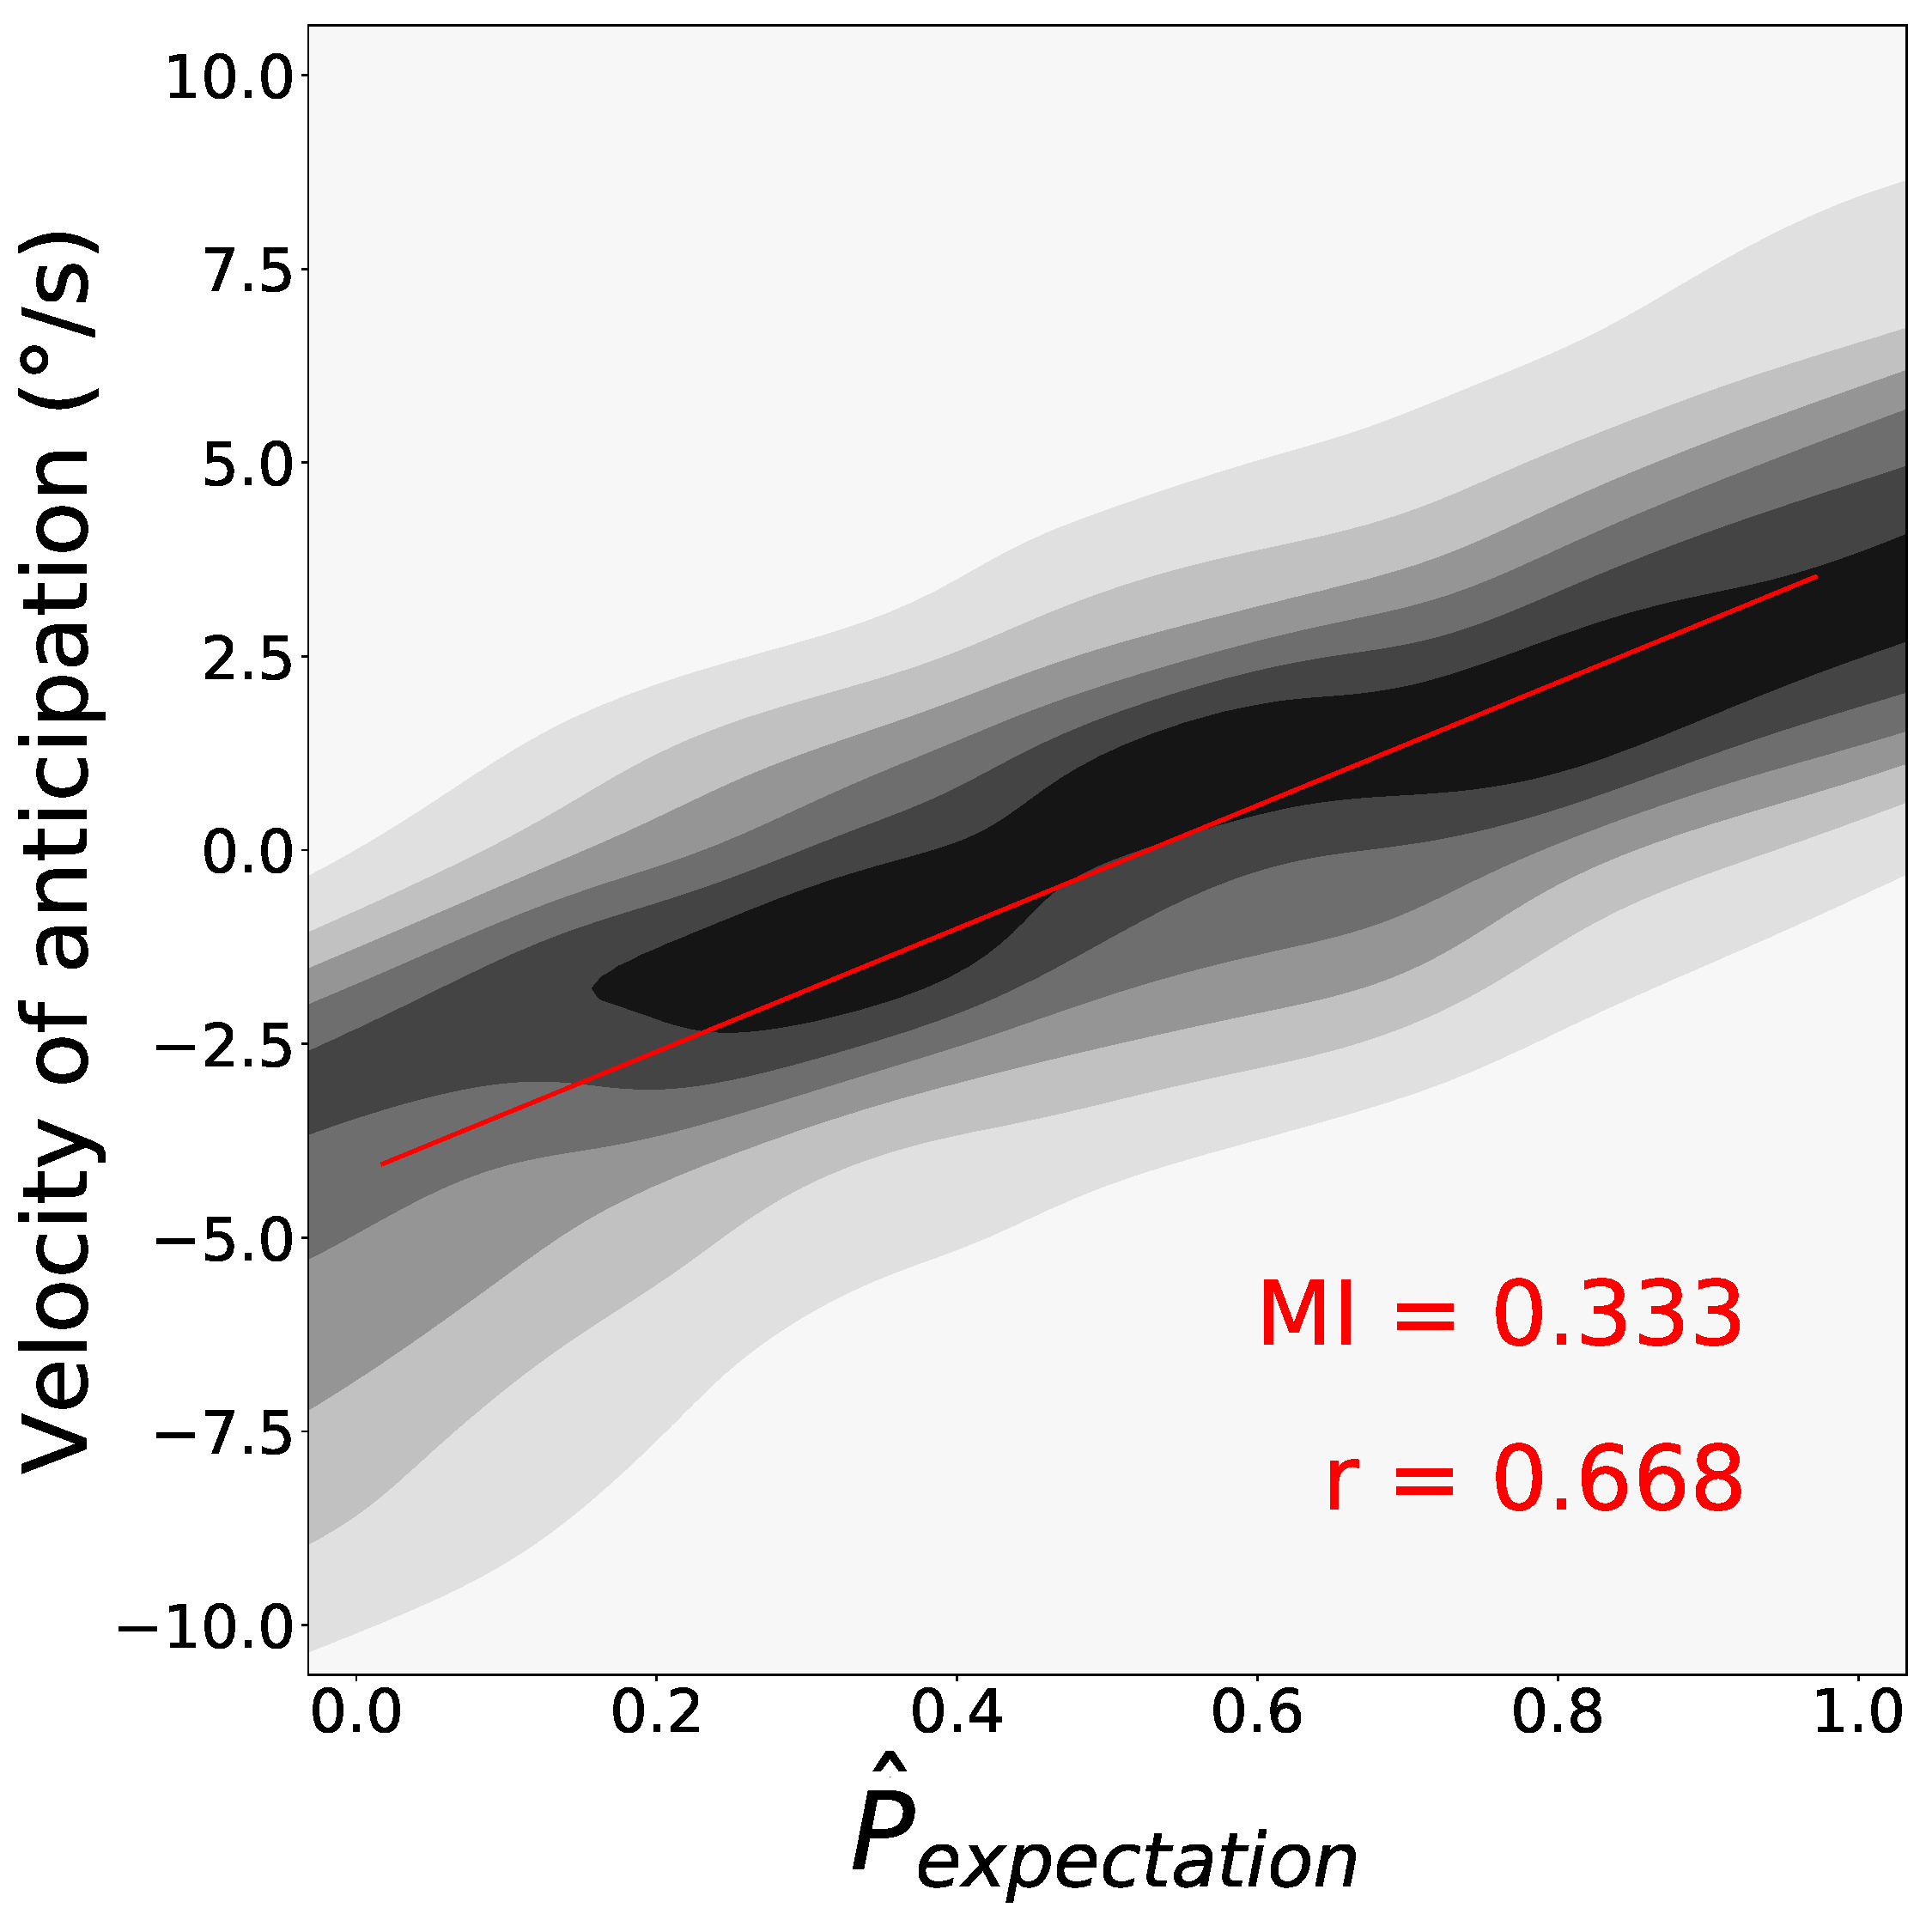
\includegraphics[width=0.49\linewidth]{4_A_result_psycho_velo}};
\node [anchor=north west]  (img4) at (0.51\linewidth,.618\linewidth){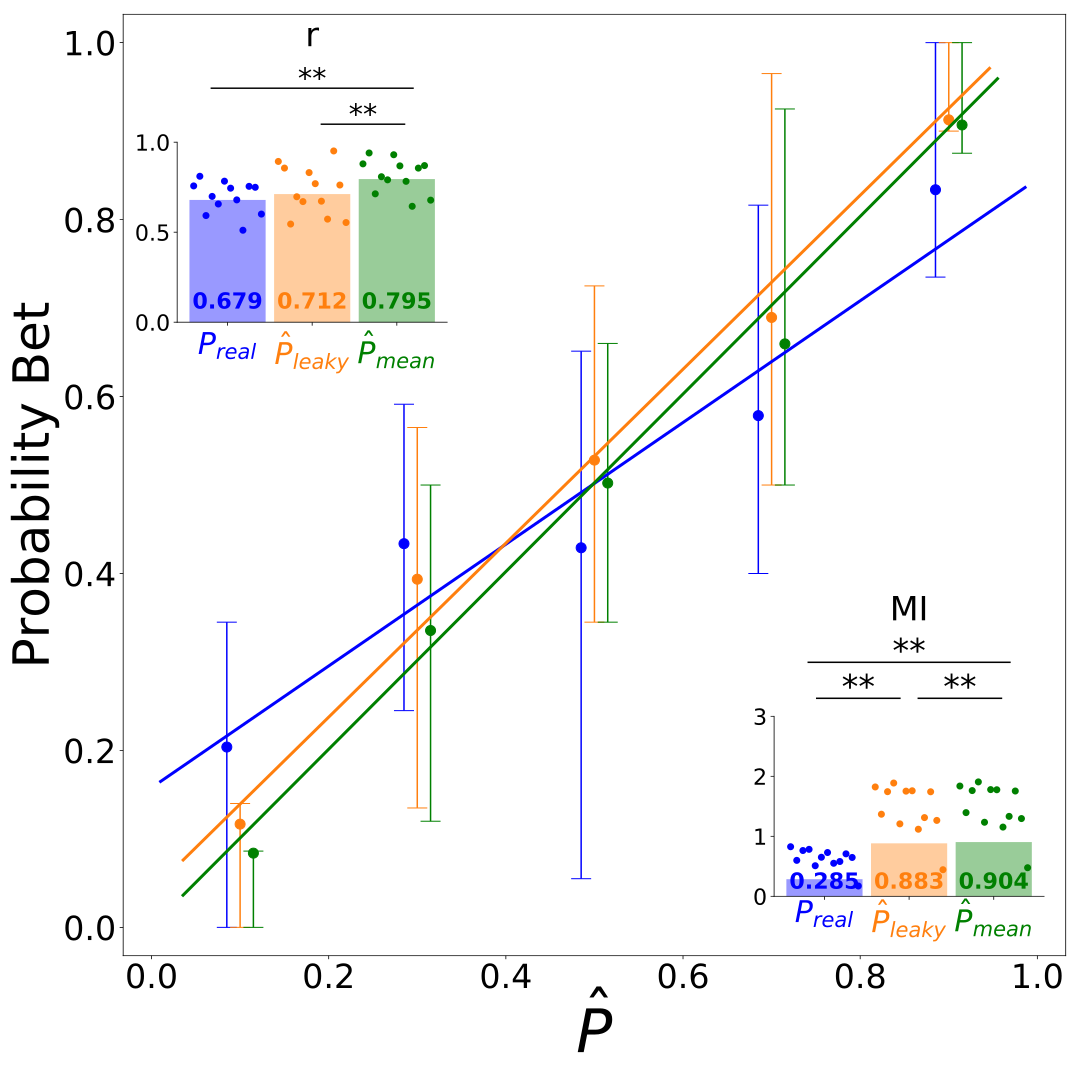
\includegraphics[width=0.49\linewidth]{4_B_result_psycho_bet}};

\draw [anchor=north west] (0.000\linewidth, .618\linewidth) node {$\mathsf{(A)}$};
\draw [anchor=north west] (0.5\linewidth, .618\linewidth) node {$\mathsf{(B)}$};

\end{tikzpicture}
}

\caption{ \emph{Psychophysical results over all participants}
\CP{Attention KDE mean !}
Each trial in our experimental results in an estimate of
the strength of aSPEM (as measured by VEM)
and a rating scale value.
Relating those values with the corresponding inferred value $\hat{p}$
of the probability bias,
this constitutes a scatter of values.
We display these relationships using a
Kernel Density Estimation (KDE) of the relationship between $p$ (abscissa)
and \textbf{(A)} VEM and \textbf{(B)} the value of bet (in ordinates).
In \textbf{(A)}, we have overlaid is a regression line which shows
a high correlation factor ($R=XXX$) which is superior to that found
with the fixed-length design (see Appendix ...)
but also with other models described in the text
(fixed-length estimator, maximum BBCP - see Appendix ... ).
In \textbf{(B)}, we have fitted the data with a logistic regression
showing a negligeable intercept (no bias) linked to the symmetry
of the problem, but a consistent slope showing an aversion to risk
(cf Kahneman13).
%\textbf{(C)}
% we should comapre with the original slope obtained by Anna?
}

\label{fig:results_psycho}
\end{figure}

%%-------------------------------------------------------------%
%: quantitive analysis
Quantitatively, we wished to look at the quality of the fit
between the strength of aSPEM and
the probability $\hat{p}$ computed by the BBCP algorithm.
In~\seeFig{results_psycho}-A, we have plotted for all subjects
this strength as a function of the inferred probability
that was coded at the second layer and which is unknown to the observer.
% TODO: First, the trend that we put in evidence is the identity of the observer
As we can see in~\seeFig{results_psycho}-A,
the probability $\hat{p}$ computed by the BBCP algorithm
is positively linearly correlated with the aSPEM velocity.
The corresponding Pearson correlation coefficient
is slightly higher than that found in
the classical experiment with fixed blocks~\seeFig{intro}-B.
Note that since the BBCP is a probabilistic model,
we can also compute the Mutual Information and
compare that value with that obtained by other models.
This analysis is presented in~\seeApp{bcp}).
This relatively strong correlation is surprising at a first sight as the probability blocks have random length,
and participants have to adapt to such a volatile environment.
However, when faced with some new observations,
the observer has to constantly adapt his response
to either exploit this information by considering that
this observation belongs to the same sub-block or to explore
a novel hypothesis.
This compromise is one of the crucial component that we wish to explore
and which is well captured by the BBCP model.
In particular, the model predicts the different facets
from the experimental results,
from the variability as a function of the inferred probability,
to the dynamics of the bahavior following a (hidden) switch.
As a consequence this leads to a stronger correlation,
as measured by the Pearson coefficient and Mutual information.
We deduce that the trace of inferred probabilities is a powerful regressor
to explain the strength of aSPEM.
We will now try to extend this result
to the second experimental session
where participants had to provide their rating scales.
%%%%%%%%%%%%%%%%%%%%%%%%%%%%%%%%%%%%%%%%%%%%%%%%%%%%%%%%%%%%%%%
\section{Results: bias rating scale measurements}
%%%%%%%%%%%%%%%%%%%%%%%%%%%%%%%%%%%%%%%%%%%%%%%%%%%%%%%%%%%%%%%
\label{sec:rating_scale}
%: qualitative analysis \seeFig{results_psycho}-B
As we could assess qualitatively in~\seeFig{results_raw}-B,
the trace of the rating scale seems to correlate well
with the inferred probability $\hat{p}$.
Similarly to the strength of aSPEM, we actually found that:
(1) The series of the paricipants' bias guesses exhibits a positive correlation with $\hat{p}$:
as a consequence, the next outcome of $x_{0}^{t}$ will in general be correctly inferred,
as compared to a random choice. %\AM{DID WE ACTUALLY PERFORM THIS COMPARISON?} - LP  it is visual / we could do it / I do not know if that would be useful...
(2) A stronger bias leads to a lower variability in the bias estimate.
(3) A (hidden) switch in the value of the bias is
most of the time correctly identified after only a few trials.
Note also that at every pause (black vertical bar in~\seeFig{results_psycho}),
participants tended to favor unbiased guesses, close to $0.5$
than at the end of a sub-block of trials.
We can speculate that this phenomenon would correspond to a resetting mechanism of the internal belief on the probability bias.
As a consequence, the experiment performed in the second session
shows that the probability-bias values that are consciously estimated by participants
are qualitatively similar to the implicit (and unconscious) ones which supposedly underlie the generation of anticipatory aSPEM with variable strength.

%: quantitative analysis
Similarly to~\seeFig{results_psycho}-A,
we now compare quantitatively the value of rating scale
as measured during the second experimental session with the model-inferred $\hat{p}$.
The KDE estimate shown in~\seeFig{results_psycho}-B,
represents the relationship between
the model-estimated probability-bias
and the rating value which was provided at each trial
by participants for the outcome of the next trial.
This analysis exhibits a consistent relationship
but which now follows a non-linear trace.
In particular, the fit was more accurate
in comparison with
the forgetful agent (see~\seeApp{results_psycho}).
We modeled this behavior as
a logistic regression over
the log-odd ratio estimated by the agent.
%TODO model this relationship by a logistic regression
This analysis provides with regression factors for each participant.
It shows that the bias (intercept)
was negligible, while the slope (logistic factor)
was always positive.
This indicates a generic aversion to risk~\citep{Kahneman13}
such that the value of a possible outcome
is down-weighted by the precision of the inference.
Our logistic regression analyses
suggests that this may come from a multiplicative weight
on the (log-) odd-ratio which is chosen as a rating scaled
compared to the (log-)odd-ratio of the inferred probability. %\AM{Is it worth to discuss more in depth the different functional dependence on p of the two experimental measures? Cite Santos and Kowler discussion about this!} - LP: that would certainly be a great addition...

%%%%%%%%%%%%%%%%%%%%%%%%%%%%%%%%%%%%%%%%%%%%%%%
\section{Results: Analyzing inter-individual differences}
%%%%%%%%%%%%%%%%%%%%%%%%%%%%%%%%%%%%%%%%%%%%%%%
\label{sec:inter}
%: separate above analysis
So far, our quantitative analysis was performed independently
for the different participants.
In particular, we have shown a representative example in~\seeFig{results_raw}
but results varied across participants (see~\seeApp{results_psycho}).
This was best characterized qualitatively in both sessions by differences
in the variability of the responses but also for instance
with different characteristic delays after a switch.
This reflects the spectrum of individual choices
between the behaviors of exploration versus exploration ~\citep{Behrens07}.
Here, we were interested in characterizing the preference
of each individual participant, but also to characterize
if this preference covaried across the two sessions.
Crucially, we have seen that the BBCP model is controlled by a single parameter,
the hazard rate, or equivalently by its inverse, the characteristic time $\tau$.
Also, we have shown that knowing an observed sequence of behavioral responses,
we could fit the best value of $\tau$ which would explain it~\seeFig{bayesianchangepoint}-C.
Thus, by extracting the parameters for every subject
we can expect to characterise inter individual differences.

%: results
%-------------------------------------------------------------%
%: FIGURE 5  fig:results_inter \seeFig{results_inter}
% TODO présente une meta analyse qui montre une correlation par sujet (scatter plot) entre h_a et h_bet (see 2017-11-16 chloe figures.pdf ) y-a-til un continuum entre explorateurs et conservatezurs?, voir de montrer une causalité entre les 2 expériences - on pourrait superposer aussi les résultats si on avait utilisé un fixed-length ?
% cf https://github.com/laurentperrinet/bayesianchangepoint/blob/master/notebooks/test_hazardrate.ipynb
% cf : 4_Meta_analysis.ipynb
\begin{figure}%[b!]
\centering{
\begin{tikzpicture}%[thick,scale=1, every node/.style={scale=1} ]
\node [anchor=north west]  (img4) at (0.000\linewidth,.588\linewidth){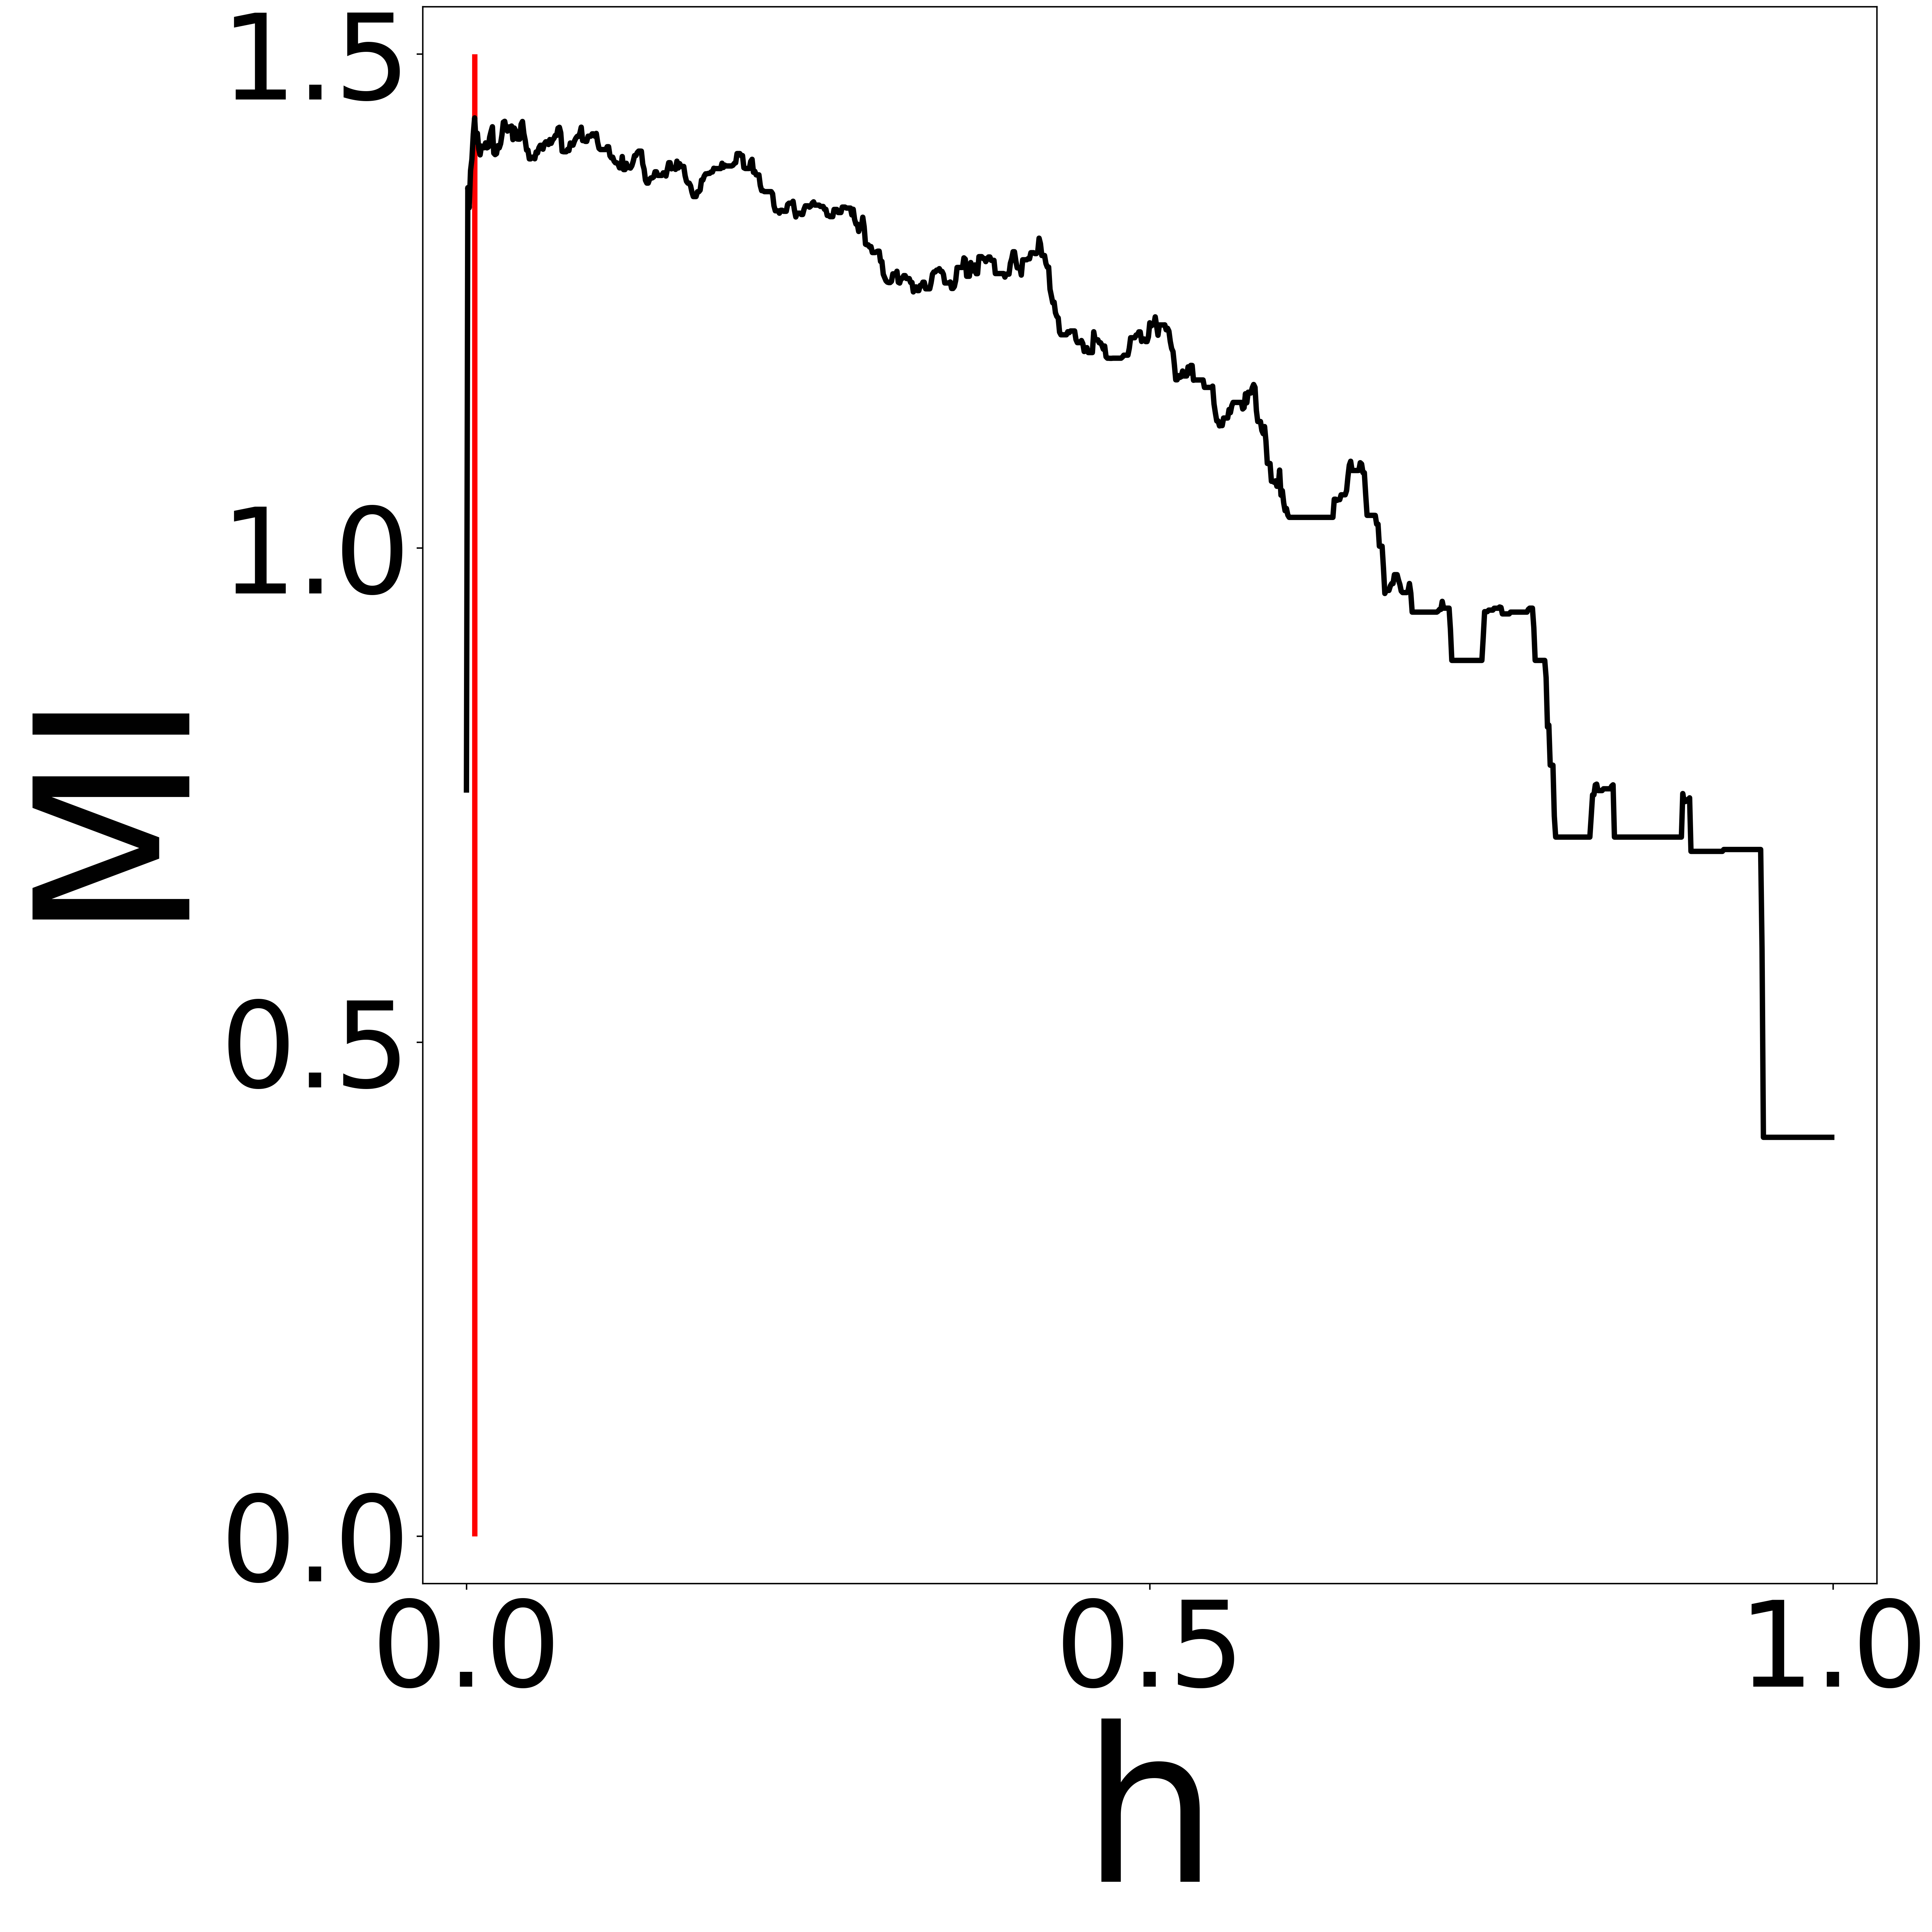
\includegraphics[width=0.25\linewidth]{5_A_h_bet}};
\node [anchor=north west]  (img4) at (0.000\linewidth,.28\linewidth){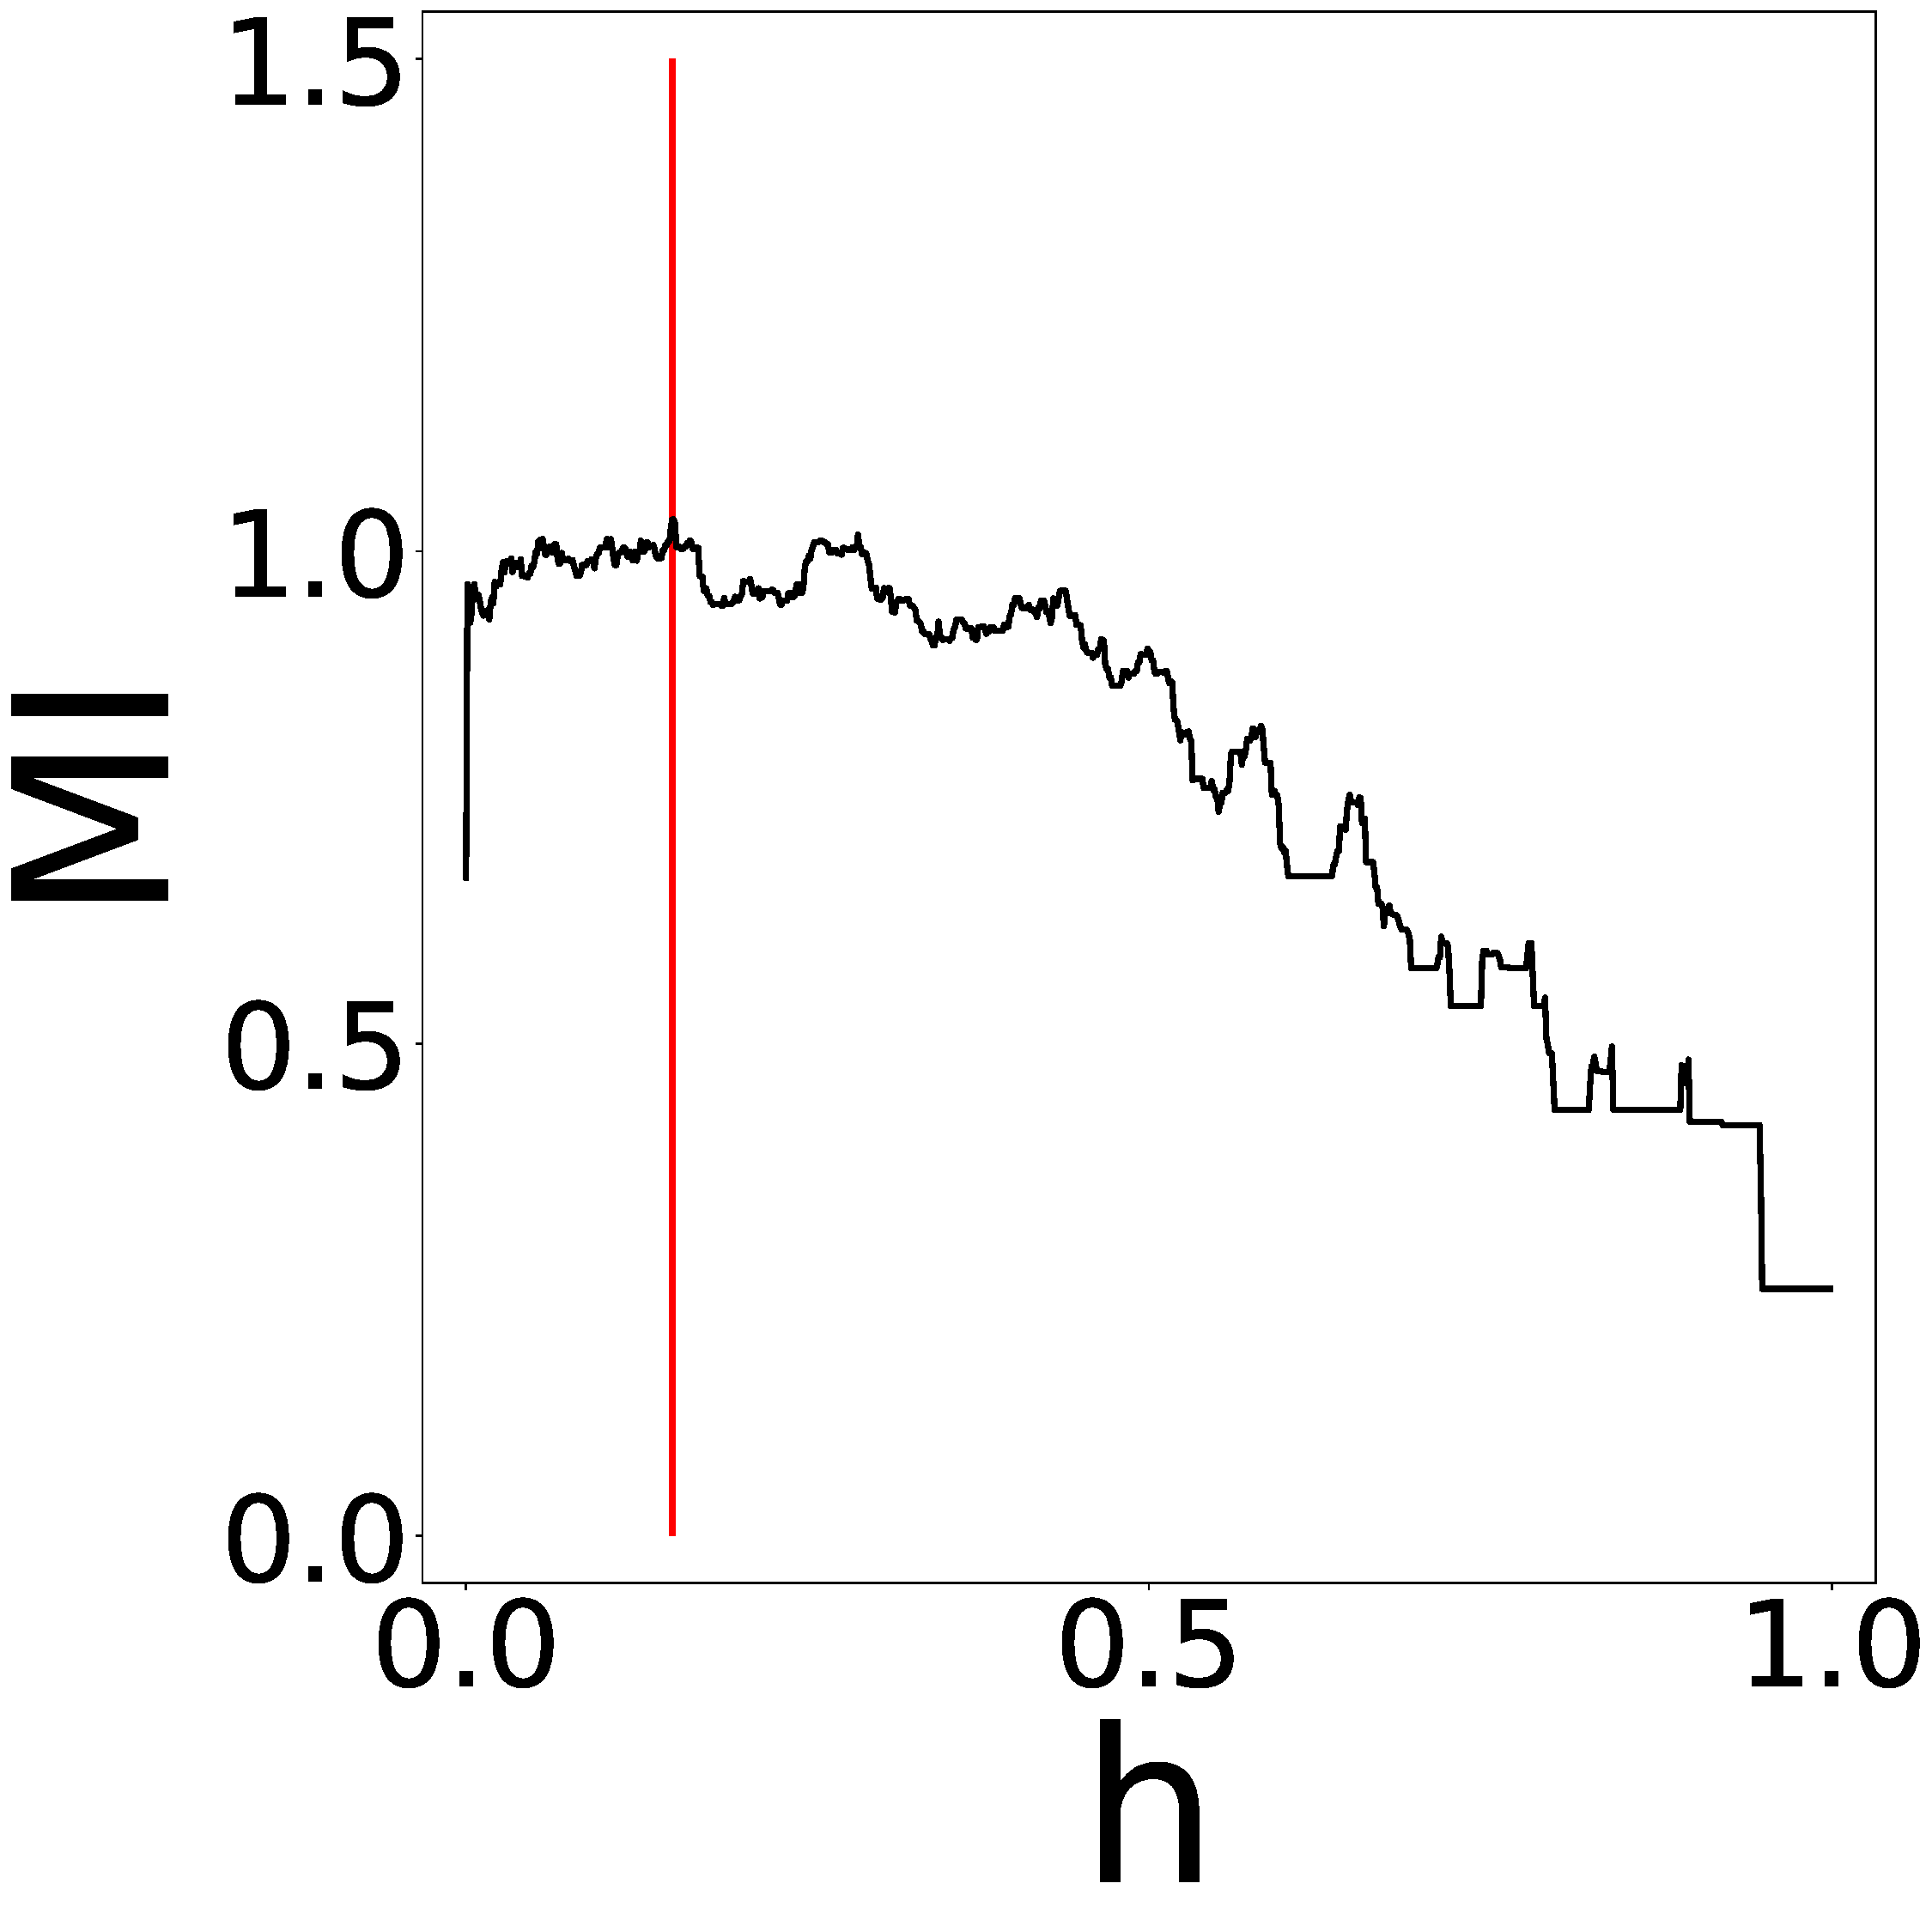
\includegraphics[width=0.25\linewidth]{5_A_h_va}};
\node [anchor=north west]  (img4) at (0.26\linewidth,.618\linewidth){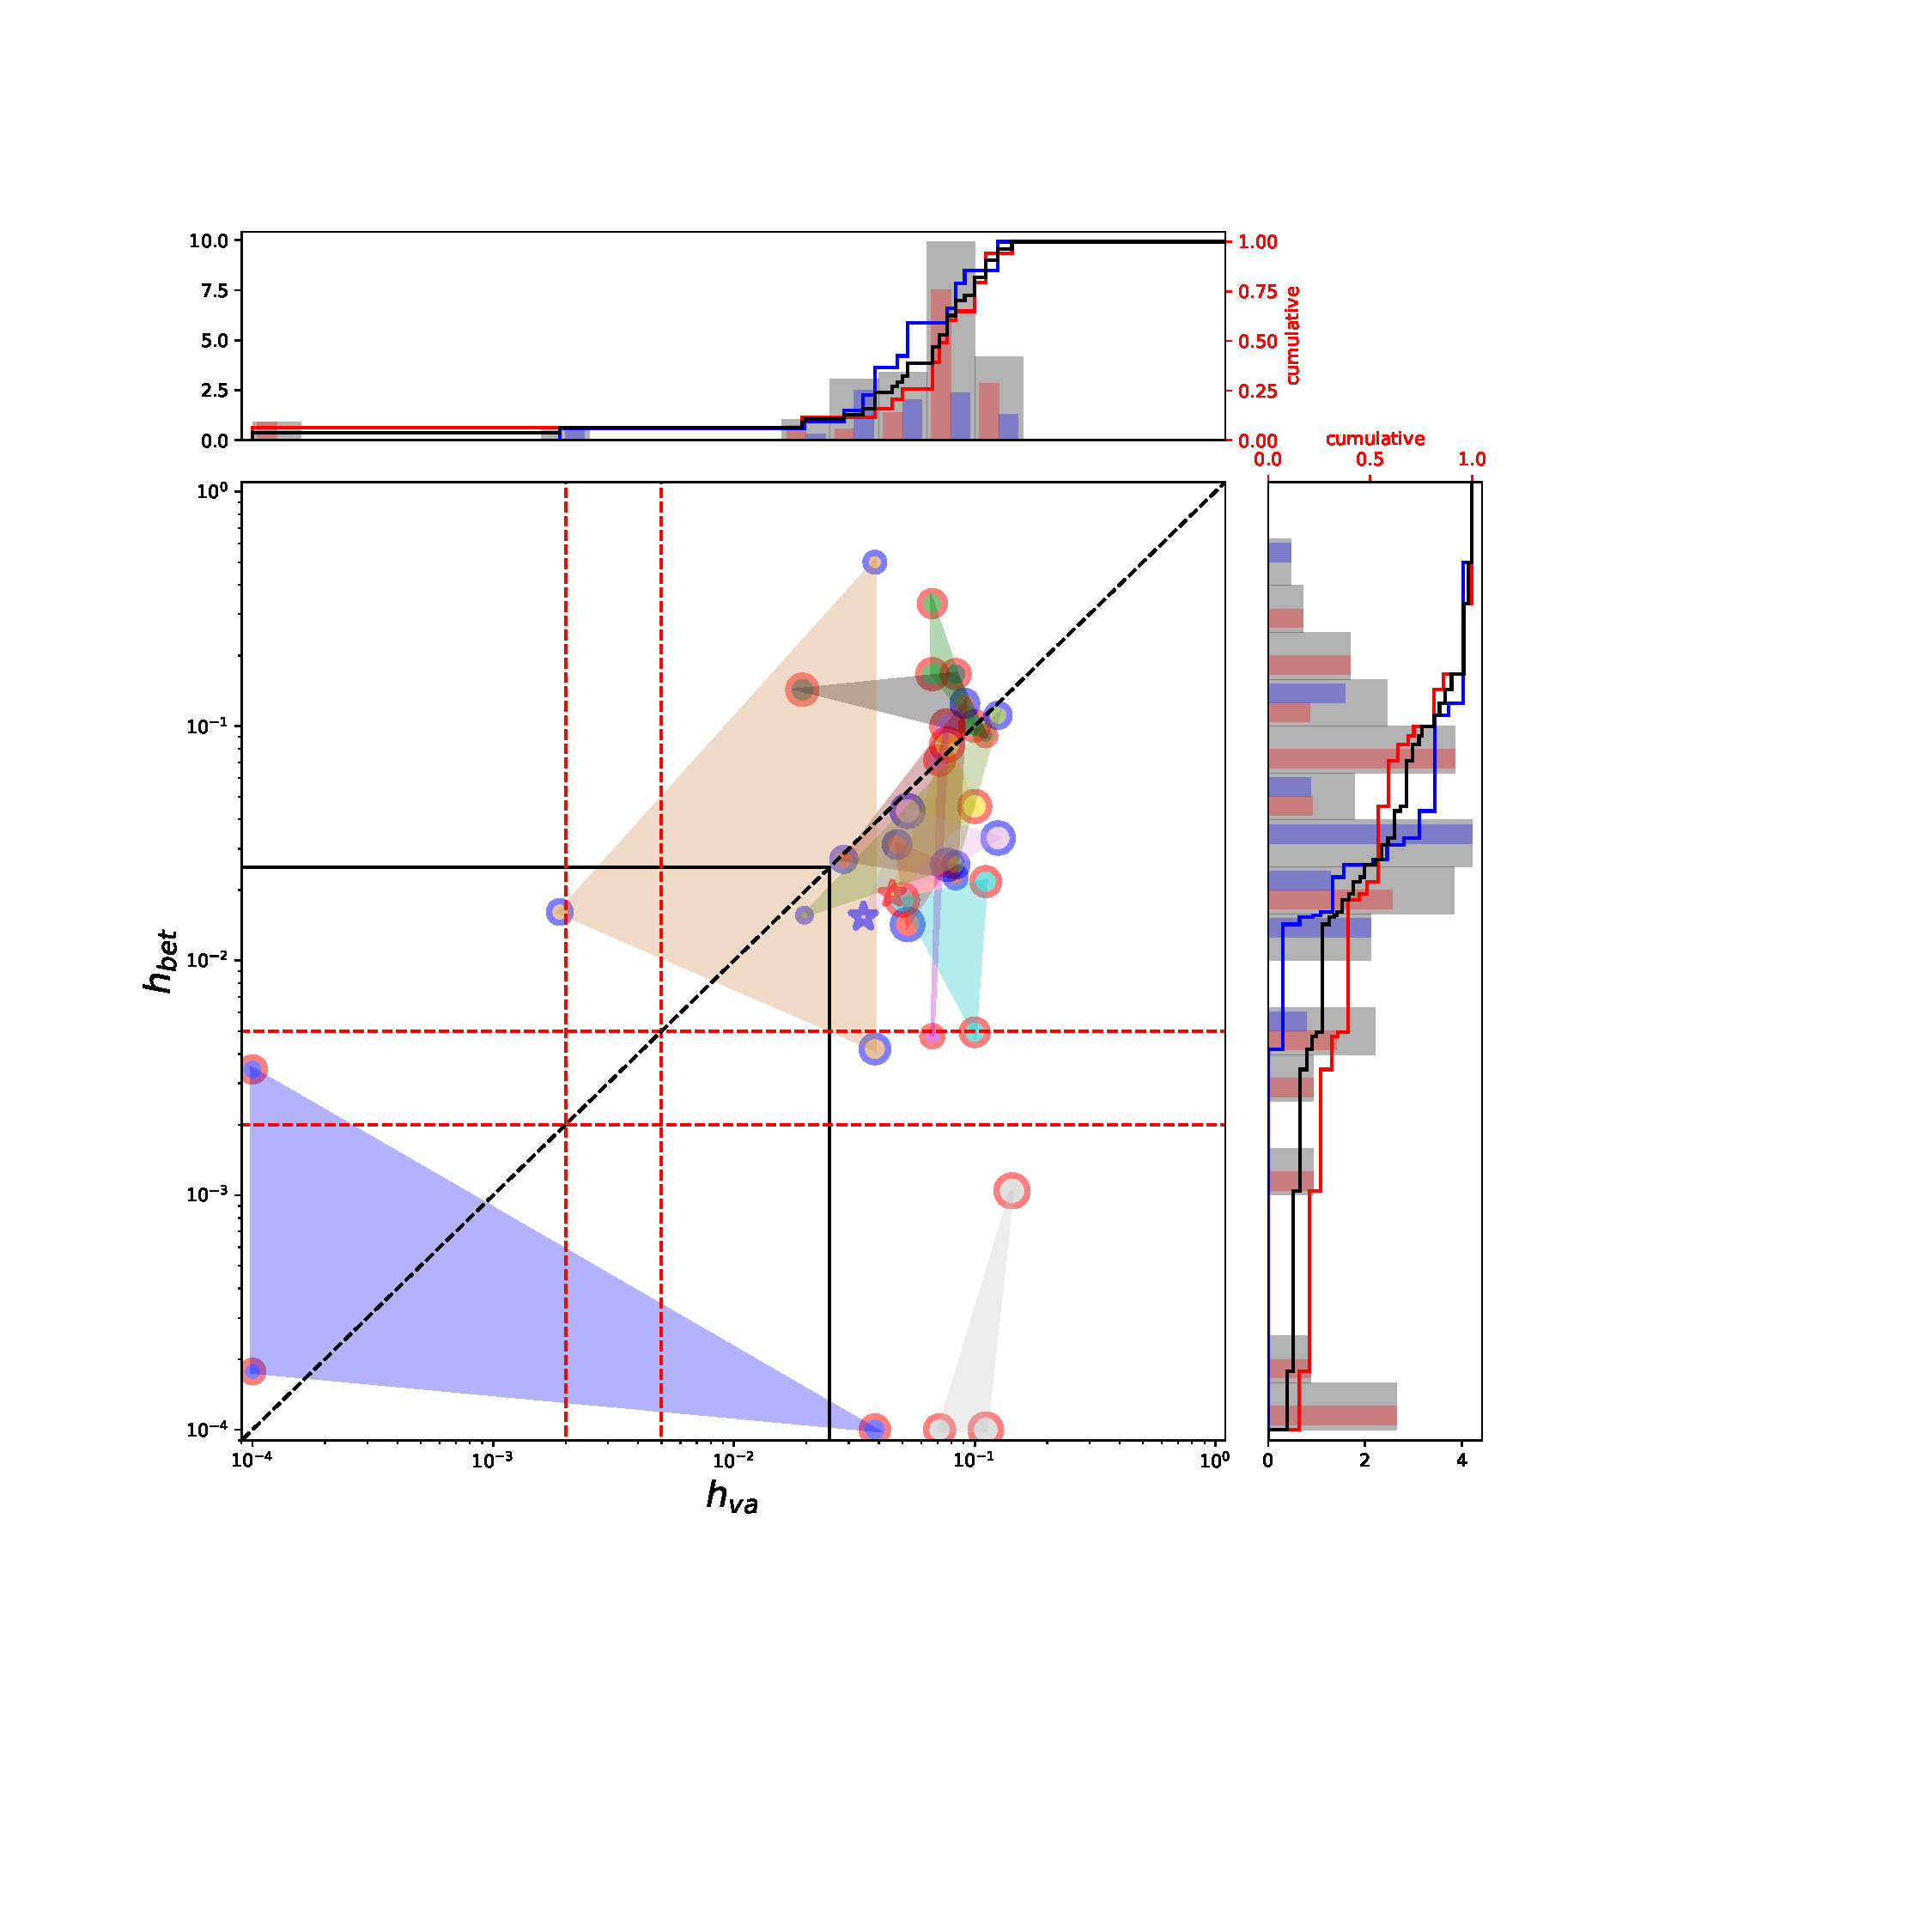
\includegraphics[width=0.618\linewidth]{5_inter-individual_differences_fit}};

\draw [anchor=north west] (0.000\linewidth, .618\linewidth) node {$\mathsf{(A)}$};
\draw [anchor=north west] (0.25\linewidth, .618\linewidth) node {$\mathsf{(B)}$};

\end{tikzpicture}
}


%\begin{figure}%[b!]
%\begin{center}
%  %\includegraphics[width=1\linewidth]{figure5}
%
%  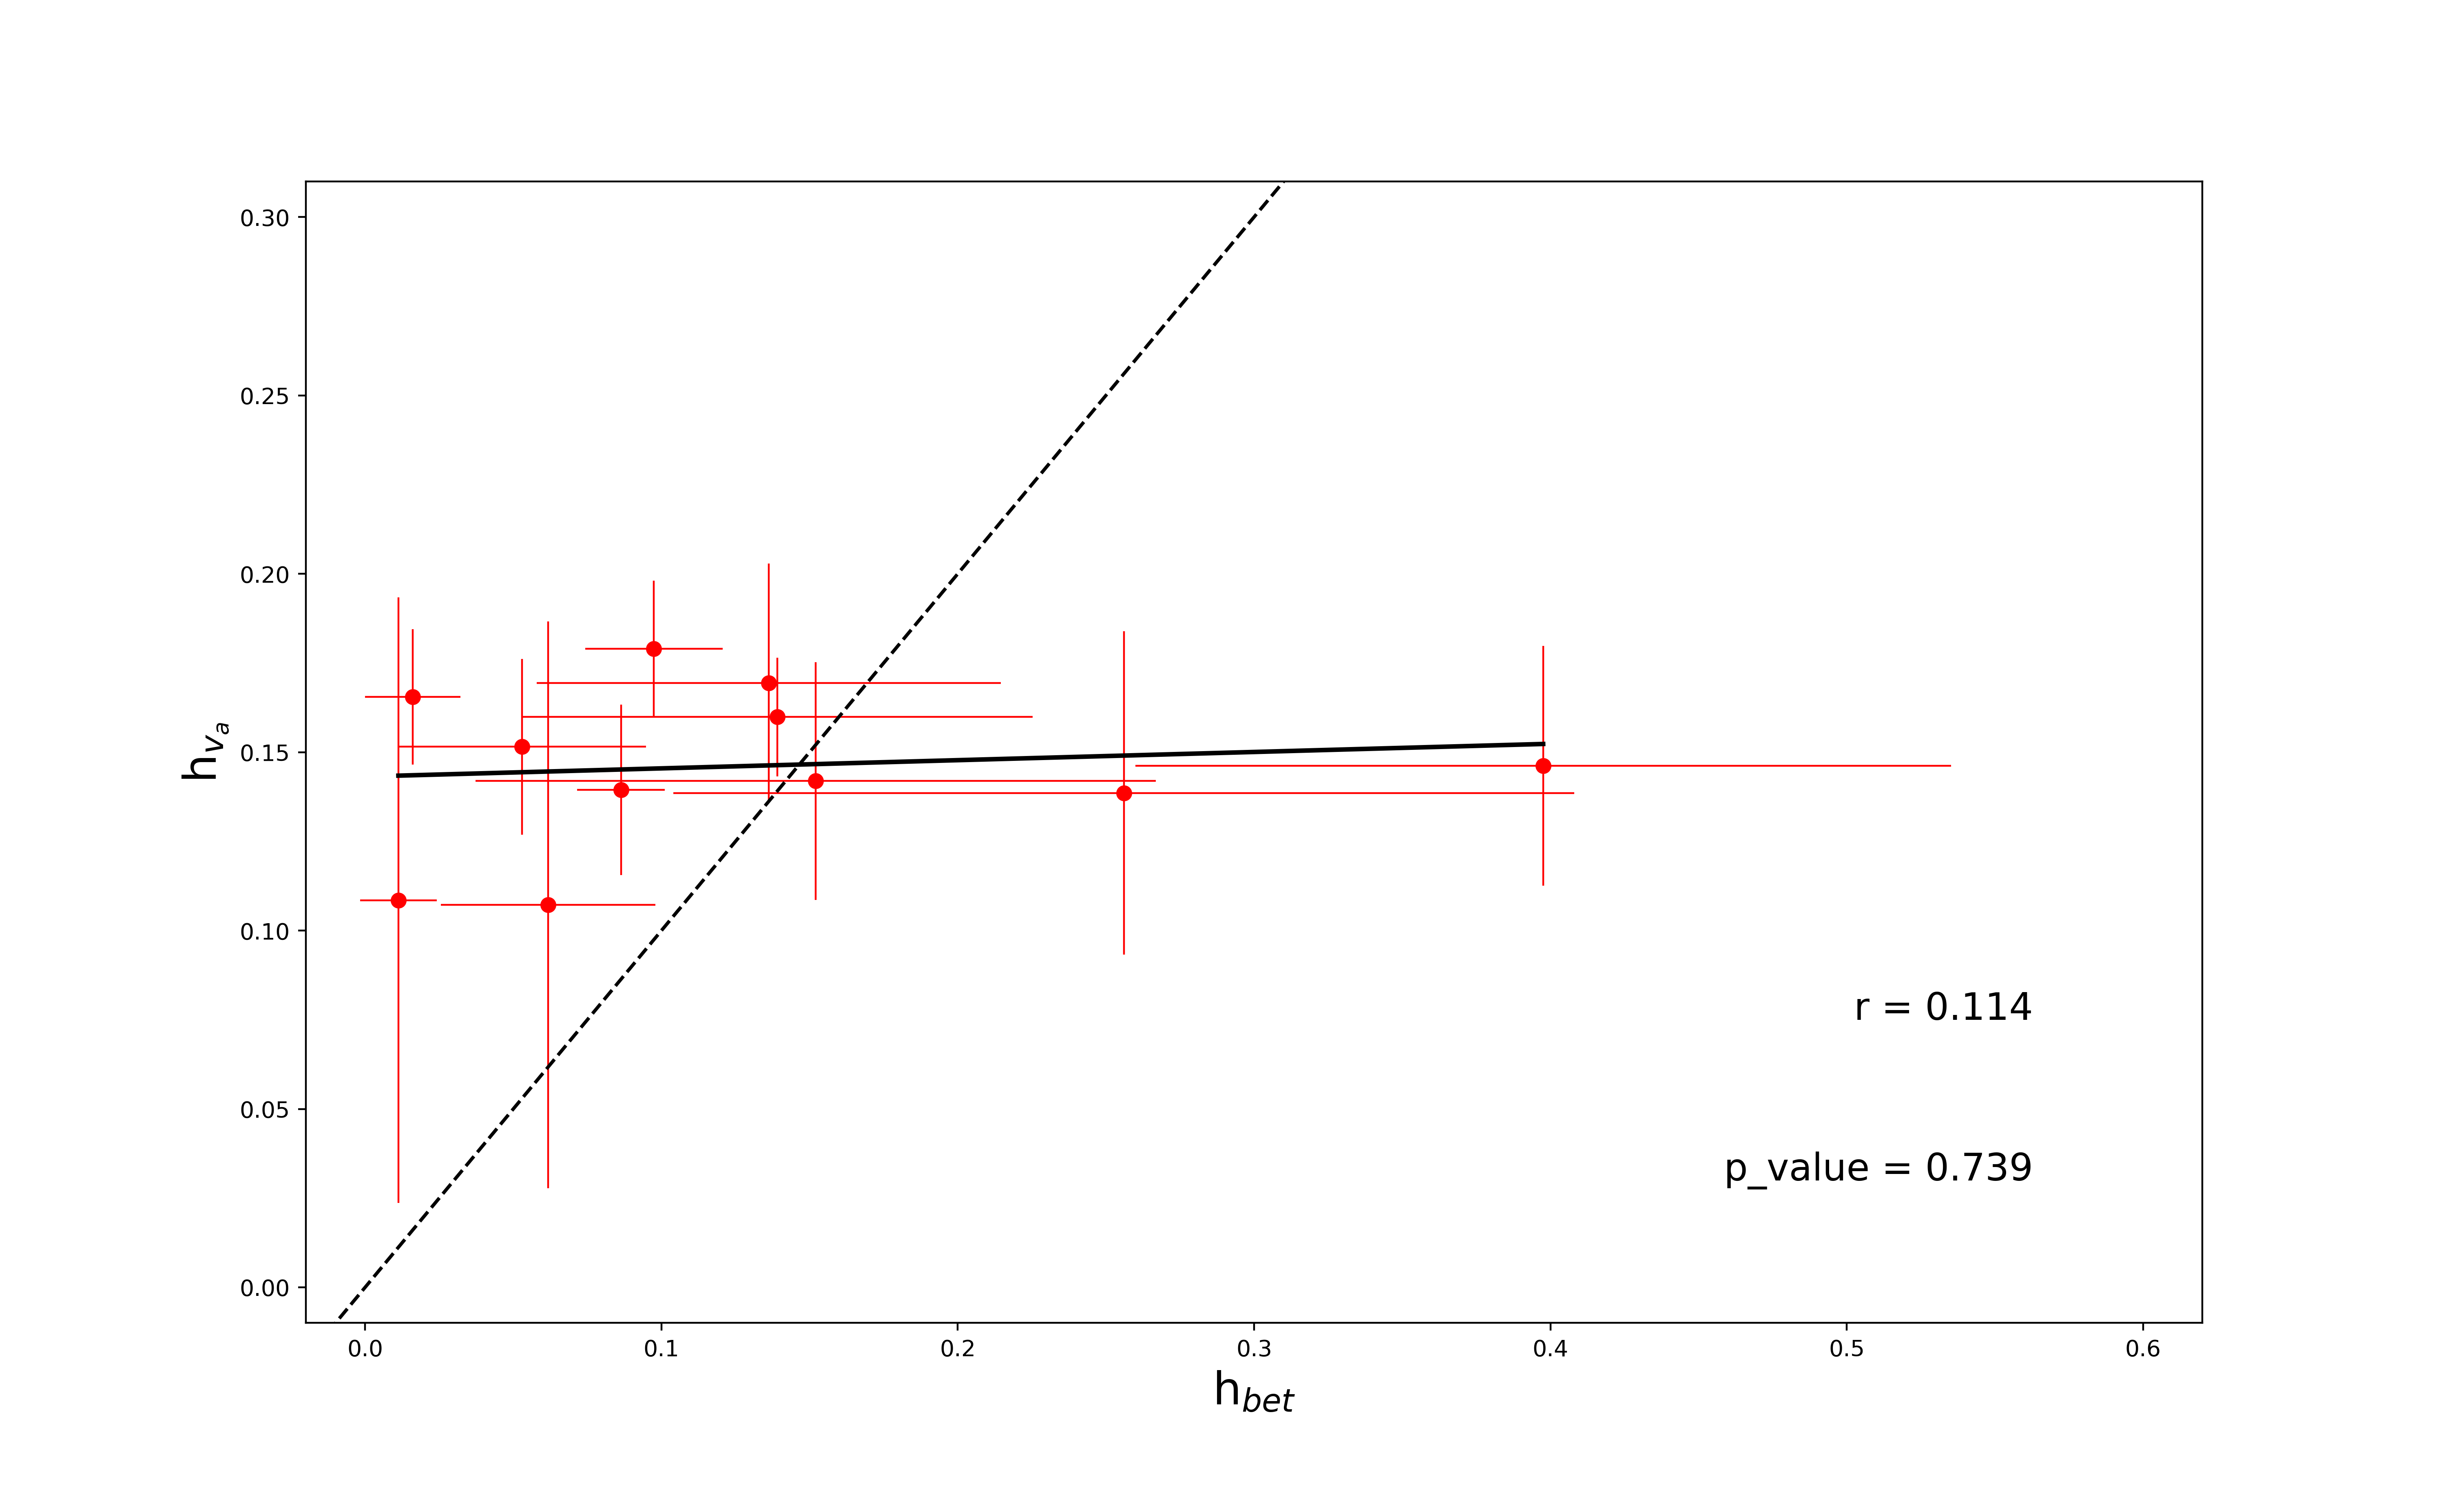
\includegraphics[width = 1 \linewidth]{5_inter-individual_differences}
%\end{center}
\caption{\emph{Analyzing inter-individual differences}
\textbf{(A)}
\LP{ show fit with different hazard rates for one observer / one block}
\CP{sujet IP 2eme block,  en haut: MI entre les bet et le bcp pour les differents h, en bas: MI entre les vitesse d'anticipation et le bcp pour different h}
% TODO compare with the results you would obtain from a fixed window fit.
\textbf{(B)}
result of fits for different observers / SEM across blocks
\CP{il y a aussi la figure pour les h selectiones avec le MI (5 inter individual differences MI)}
}
\label{fig:results_inter}
\end{figure}
%-------------------------------------------------------------%
Hence, we have fitted the sequence of responses generated by each participant and
for each session, that is for the eye movements and the rating scale experiments.
The scatter plot of the best fit values are shown in~\seeFig{results_inter}.
This figure suggests, in the first place, that there is some variability in the best fit value of $\tau$
in both sessions.
If the average is close to the (hidden) value used to generate the sequence
(with $\tau = XX~\ms \pm XX~\ms$ for the first session and
 $\tau = XX~\ms \pm XX~\ms$ for the second),
 we observe a variability which is characteristic of the spectrum of individual choices.
More importantly, there is a small but consistent
correlation between the individual best-fit values estimated for the first and the second session.
% TODO - Granger / transfer entropy
Also we have found that using measures of causality %\AM{COOL!}, LP: yaka :-)
the results for eye movements slightly lagged before
that of the rating scale,
suggesting that there could be an advance
It can serve as a biomarker...

%: %%%%%%%%%%%%%%%%%%%%%%%%%%%%%%%%%%%%%%%%%%%%%%%%%%%%%%%%%%%%%%%

\section{Discussion}

\label{sec:outro}

%The oculomotor system has to constantly update its knowledge about the environment. An ordeal is then to adapt to changes with the shortest delays. Early studies have proposed that stimuli provides information to modulate reaction times within sequences~\citep{Hyman1953, Tune1964, Schvaneveldt}. This theoretical approach is coherent with the notion of local transition probabilities that quantifies at which extent an observation deviates from the preceding ones~\citep{Meyniel16}. The way expectations act on cognitive processes has been investigated by a wide range of domains such as predictive coding~\citep{Wolpert2000, Wacongne2012}, active inference~\citep{Friston2010}, motor control~\citep{Sutton1998, Behrens07} and reinforcement learning~\citep{Nassar2012}. Non-stationary observations can also explain why both local and global effects emerge and why local effects persist in the long run even within purely random sequences~\citep{Cho2002, Yu2009}. This constant update of a general belief on the world can be a consequence of the constant attempt to learn the non-stationary structure of the environment that can change at unpredictable times~\citep{Yu2009}. Many studies have actually already pointed the brain's ability to apprehend non-stationary states in environments~\citep{Ossmy2013, Meyniel15}. As explained by~\citet{Meyniel16}, the belief upon an environment can be divided in two different ways:
%
%\begin{enumerate}[label=\Alph*)]
%\item Update the~\textit{a priori} likelihood of a sudden change, also known as the volatility and taken into account by the model~\citep{Behrens07}
%\item A leaky integrator factor imbedded in the model~\citep{Anderson2006, Yu2009, Ossmy2013, Wang2002}
%\end{enumerate}
%

%: theory / computationnally-driven experiments
% it's a main novelty
generative models for changing environments allows to know the ground truth compared to natural stimulation (see Rust eand Movshon)%
Let's remember our hierarchical generative model.

At any given trial, we wish to construct an algorithm which

We will introduce a fundamental component of Bayesian models : a latent variable

this new variable will be used to test different hypothesis which will be evaluated to predict future states. it is called latent because it aims at representing a variable that is latent (or hidden) to the observer

in our case, we will assume that the Bayesian model knows about the structure of the generative model and we will set it to the current run-length $r$, that is, at any given trial, the hypothesis that the past r observations belong to the same block. of course a wrong choice of a latent variables (let's say the temperture in the experimental room) may give unexpected results, even is the Bayesian model is ``optimal'' - an essential point to understand in Bayesian inference

extension to multi-nomioal( daniele + fred danion)



% Still, only Bayesian models recover an explicit probabilistic representation of change in likelihood. Recent experimental studies suggest, indeed, that the brain is able of estimating a hierarchical model of the environment and that humans can explicitly report sudden changes in sequences~\citep{Meyniel15, Gallistel2014}. Ultimately, we passed over one of leaky integrator models' main default, having a too fixed and rigid memory parameter. In our work the memory parameter is constantly inferred by the BBCP algorithm over the observation of the number of trials where this inference stayed reliable and then globally represented probabilistic representation of changes in likelihood and actualization of~\textit{a priori} knowledge.


perspectives:
- RL : use hindsight example of localization for saccades: get the changepoints then improve estimate of reward allows to optimize the association between the set of measures and their utility (compared to Q-learning where it is a fixed length)
- interindividual differences : markers for the berhaviour traces - traces of the network implementation / testing different h
- the brain is weakly Bayesian (it does not care about equations but more about sugar)


One remaining question though, is to understand why in cognitive systems
this adaptation occurs and
in particular why it may deviate
in some pathological disorders such as schizophrenia~\citep{Adams12}.

%: %%%%%%%%%%%%%%%%%%%%%%%%%%%%%%%%%%%%%%%%%%%%%%%%%%%%%%%%%%%%%%%

\section{Conclusions}


\begin{itemize}\setlength{\itemsep}{0ex}
\item There is a strong correlation between the real probability and the value of the bet,

\item there is a stong correlation between the strength of anticipation and the probability of the process,

\item we have developed a Bayesian model of an agent estimating the probability of changing points. This allows to dynamically infer the direction probability and directly compare model and human behaviour.

% to summarize, we have shown that
% - there is a correlation in the anticiapatory response of eye movements
% in a volatile environment that is captured if we know the true probability
% - that a fixed length models captures some of this correlation, but that
% - our online bayesian changepoint model better captures this correlation
% and that this may hint at the neural mechanisms used to anticipate
% in a dynamic environment
%
% the brain is not strongly a bayesian machine, but weakly

\end{itemize}
%: %%%%%%%%%%%%%%%%%%%%%%%%%%%%%%%%%%%%%%%%%%%%%%%%%%%%%%%%%%%%%%%
\section{Material and Method}
%%%%%%%%%%%%%%%%%%%%%%%%%%%%%%%%
%%%%%%%%%%%%%%%%%%%%%%%%%%%%%%%%
\subsection{Psychophysics}
%%%%%%%%%%%%%%%%%%%%%%%%%%%%%%%%



% TODO replace this with the actual protocol using psychopy

%cf. https://github.com/chloepasturel/AnticipatorySPEM/issues/19
\textbf{Stimuli were generated using PsychoPy 1.85.4 on a Mac running OS 10.6.8 (A VERIFIER) and displayed on a 20" Viewsonic p227f monitor (A VERIFIER) with resolution $1280\times 1024$ at 100~\si{\Hz} (60 ?). Psychophysics routines were written using PsychoPy 1.85.4 controlled the stimulus display. Observers sat 57~\si{\cm} from the screen in a dark room. Twelve observers (29 years old +/- 5.15) with normal or corrected-to-normal vision took part in these experiments. They gave their informed consent and the experiments received ethical approval from the Aix-Marseille Ethics Committee in accordance with the declaration of Helsinki.}
%Stimuli were presented on a 21 inches CRT monitor with refresh rate of 100 Hz. Stimuli were generated using the Psychophysics Toolbox extension for Matlab (Brainard, 1997; Pelli, 1997) running on a Mac Pro (first generation) computer and displayed at a viewing distance of 57 cm against a gray background. The luminance of the gray background was 42 cd/m2. To minimize measurement errors, the subject’s head movements were restrained using a chin and forehead rest, so that the eyes in primary gaze position were directed towards the center of the screen. Eye movements were measured continuously with an eye tracking system (Eyelink 1000, SR Research Ltd., sampled at 1000 Hz) and data were transferred, stored, and analyzed offline using programs written in Matlab or Ipython notebooks.
%Recorded horizontal and vertical gaze position were low-pass filtered using a Butterworth (acausal) filter of order 2 with a 30 Hz cut-off frequency and then were numerically differentiated to obtain velocity measures. We used an automatic conjoint acceleration and velocity threshold method to detect saccades (Krauzlis & Miles, 1996) and further inspected all individual traces visually to exclude aberrant trials. Saccades were excluded from eye velocity traces (and replaced by NaN values in the numerical arrays) before trial averaging. We evaluated the effects of the experimental manipulations on anticipatory velocity at the individual level, by comparing the mean eye velocity during a critical time window, between –50 and +50ms around target motion onset (as highlighted in Figure 2), using individual one-way ANOVAs (with the probability bias or reinforcement type as 3-levels single factors). We also computed all post-hoc pair-wise comparisons using Tukey’s HSD test. Even though the normality assumption of our data was fairly justified given the sample’s size (always over 60 trials per condition), we also computed non-parametric statistics (Kruskal-Wallis test) for comparison and results were similar. All tests and analyses have been realized using Python 3.5 with the Numpy and Scipy libraries.
3 blocks of 200 trial - with 4 sub-blocks of 50 trials


 * the whole experiment was coded by Chloé using :
 - python for the generative model,
 - the psychopy library for the stimulus display + connection to the eyelink 1000 that we used to record EMs
 - numpy, pandas and pylab for the data analysis

  * all this code is available : for running the experiments, re-analyzing the data and doing all plots are on github

These python scripts are available at \url{https://github.com/chloepasturel/AnticipatorySPEM}.


We asked subjects to perform two tasks on different days :
%\begin{itemize}\setlength{\itemsep}{0ex}
%\item a <<Bet>>
%\item a <<recording>>
%\end{itemize}

In summary, the design of our experimental setting is therefore very similar to the previous experiment but with a more general construct:

- using the same 3-layered generative model, we generated sequences of directions

- and generated 3 blocks of 200 trials

- with an average block length of 40 trials

We anticipated that such an  experiment for which we simply recorded the eye movements should be more difficult for observers compared to the classical experiments with longer (400 trials), fixed blocks and...

\subsection{The Bet}
In this first part, the subjects must simply answer before each trial at the question \textit{ ``How sure are you that the target will go left or right''}. This was performed by adjusting a cursor on the screen using the mouse (see Figure).

%\textbf{ Un point de fixation blanc de 10px de large est affiché au début d'un essai. Les sujets doivent ajuster le curseur sur une échelle blanche gradué placé en desous. Cette échelle présente 3 graduations : 'gauche' et 'droite' au extrémité et 'incertain' au millieu. Pour validé leurs choix, les sujets doivent cliquer sur la souris. L’échelle et le point de fixation disparaissent et une cible en mouvement à 15°/s (voir pour LB$_Bet$ 20°/s) s’affiche à l’écran. La cible est un cercle blanc mesurant 10px de large et 2px de lineWidth.}


%\textbf{Lors de cette tâche les mouvement oculaire sont enregistré à 100 Hz via Eyelink 100. Le module Python Pylink (SR research) 0.1.0 nous a permis de faire le lien entre Eyelink et nos routines python. Les sujets ont la tête fixe, et on leur demande de ne pas cligner des yeux lorsque le stimuli aparait. Chaque essais commence par la présentation d’un point de fixation blanc de 10px de large au centre de l’écran pendant une durée variable de 400 à 800 ms. Si le signal enregistré n'est pas présent dans une fenêtre de $120\times 120$ px autour du point de fixation ou si il n’est pas stable (clignement, mauvais enregistrement…), la durée de fixation recommence. À la fin de cette durée de fixation il y a un GAP de 300ms, le point de fixation disparait laissant juste un écran gris. Puis une cible en mouvement de 15°/s apparaissait de sorte que 100ms après sont apparition il soit au centre de l’écran, afin d’évité la première saccade. La cible est un cercle blanc mesurant 10px de large et 2px de lineWidth (REDONDANT).}


This is why we added a supplementary experiment for each observer but on a different day for which we asked at every trial to give a subjective, conscious evaluation of the direction of the next trial + a confidence about this inference. Once this information given by the subject, we were showing the actual outcome.

Interestingly, we used exactly the same sequence, allowing to make a direct comparison of the results of both experiments

We called this experiment the bet experiment.


\textbf{Tous les 50 essais le 'score' du sujet sur les 50 derniers essais est affiché au centre de l'écran, le sujet doit appuyer sur la barre espace du clavier pour continuer (doit dire a l'expérimentateur quand il veux continué, on ne pouvais pas brancher une souris et un clavier en même temps). Ce score est égal à $\sum_{x=0}^{50} \frac{Bet_{x} \times dir_x}{50} \times 100$. Où $Bet_x$ est le parie du sujet à chaque début d'essaie comprie entre -1 pour la gauche et 1 pour la droite, $dir_x$ est la direction de la cible pour chaque essai, -1 pour la gauche et 1 pour la droite.}


%\subsection{The Bet}
%Example of results obtained during the bet :
%\begin{center}
%    \includegraphics[width=1\linewidth]{results_pari}
%\end{center}
%%Comparison of probabilities bet with respect to the real probability :
%The scatter plot of the value of the bet (probability bet) as a function of the real probability at every given trial shows that there is a good correlation between both values:

%\begin{center}
%    \includegraphics[width=1\linewidth]{p_real--p_bet}
%\end{center}

\subsection{Eye movements recording}

%
%Experiment 1: motion direction-bias task (Baseline)
%	 The visual stimulus used in experiment 1 was a white ring (0.30° outer diameter and 0.23° inner diameter) with a luminance of 102 cd/m2 that moved horizontally on a grey background. Each trial started with a central fixation point displayed for a random duration drawn from a uniform distribution ranging between 300 and 600ms. Then a fixed-duration 300ms gap occurred between the offset of the fixation point and the onset of the moving target, which was presented at the fixation location and immediately started moving horizontally at a constant speed of 7.7 °/s, either to the right or to the left for 1000 ms. Across experimental sessions, the probability P of rightward trials was manipulated in order to create a direction bias and favor the buildup of direction expectancy (See Figure 1A). The experiment included three sessions. The first session had P=0.50, hence about 200 rightward trials out of 400 trials; the second one had P=0.75 (about 300 rightward trials out of 400 trials); the last one P=0.90 out of a total of either 400 (360 rightwards) or 600 trials (540 rightwards) (respectively 9 and 10 participants). The rationale for having a larger number of trials in the P=0.90 session was to collect enough trials for the least frequent direction, namely the left one, but after running the first participants, we realized that the detailed analysis of the least-frequent trials did not provide per se a major advantage for the present study, since the anticipatory behavior was clearly observable with the standard 400 trial-sessions. As we wanted to test a condition without any direction uncertainty, four participants also completed an additional session of 400 rightward trials only (P=1.00). With the exception of the P=1 condition, target motion direction was pseudo-randomized across trials once for each session type, such that all participants were presented with the exact same sequence of randomly alternating directions. Participants were instructed to track the target as accurately as possible.
%
%
Then, we recorded their eye movements as they were tracking the target's motion. Importantly, we used that exact same sequence.

% TODO replace this with the actual protocoml using psychopy
%Stimuli were generated using Matlab 7.10.0 on a Mac running OS 10.6.8 and displayed on a 20" Viewsonic p227f monitor with resolution $1024\times 768$ at 100~\si{\Hz}. Psychophysics routines were written using Matlab and Psychtoolbox 3.0.9 controlled the stimulus display. Observers sat 57~\si{\cm} from the screen in a dark room. Six male observers with normal or corrected-to-normal vision took part in these experiments. They gave their informed consent and the experiments received ethical approval from the Aix-Marseille Ethics Committee in accordance with the declaration of Helsinki.

In parallel, we are developing new automatic routines for the advanced analysis of oculomotor traces. In order to extract the relevant parameters of the oculomotor responses (latency, gain, initial acceleration, catch-up saccades), we developed new tools based on best-fitting procedure of predefined patterns (i.e. the typical smooth pursuit velocity profile).

These python scripts are available at \url{https://github.com/invibe/ANEMO}.


\subsection{Eye movements analysis}

In order to extract the relevant parameters of the oculomotor responses, we developed new tools based on a best-fitting procedure of predefined patterns and in particular the typical smooth pursuit velocity profile that was recorded for the aSPEM (Top row). This was applied to each trial individually, and we show below some prototypical example of respectively a neutral, anticipatory positive and anticipatory negative aSPEMs examples (respectively second to bottom rows).
%%%%%%%%%%%%%%%%%%%%%%%%%%%%%%%%
%: %%%%%%%%%%%%%%%%%%%%%%%%%%%%%%%%%%%%%%%%%%%%%%%%%%%%%%%%%%%%%%%
\section{Appendices}
%%%%%%%%%%%%%%%%%%%%%%%%%%%%%%%%
%%%%%%%%%%%%%%%%%%%%%%%%%%%%%%%%
\subsection{Appendix 1: Analysis of eye movements}
\label{app:em}
%%%%%%%%%%%%%%%%%%%%%%%%%%%%%%%%




I show here a typical velocity traces for one subject / 2 trials

- x-axis is time in milliseconds aligned on target onset,
and we show respectively from left to right the fixation in gray,
the GAP in pink (300ms) and the run in light gray.

- y-axis is the velocity as computed as the gradient of position.
Remark that the eyelink provides with the periods of saccades or
 blinks that we removed from the signal. it is quite noisy and
 to complement existing signal processing methods,
 Chloe implemented a robust

- fitting method which allows to extract some key components of
the velocity traces: maximum speed, latency, temporal inertia ($\tau$)
 and most interestingly acceleration before motion onset.
 We cross-validated that this method was givinfg similar results
  to other classical methods but in a more robust fashion/

While being sensible to recording errors, this allows us to extract the
 anticipatory component of SPEMs and..

%%%%%%%%%%%%%%%%%%%%%%%%%%%%%%%%
\subsection{Appendix : leaky integrator}
\label{app:leaky}
Given a series of observations $\{x_0^i\}_{0\leq i \leq t}$
with $\forall i, x_0^i \in \{0, 1 \}$, we defined
\eqs{
\hat{x_1}^{t} &= 1/\tau \cdot \sum_{0\leq i \leq t} (1 - 1/\tau)^{i} \cdot x_0^{t-i}\\
			  &= h \cdot \sum_{0\leq i \leq t} (1 - h)^{i} \cdot x_0^{t-i}
}
%is true for $t=1$: by definition $\hat{x_1}^{0}=x_0^0$ and
%\eq{
%\hat{x_1}^{1} = (1 - \rho) \cdot \hat{x_1}^{0} + \rho \cdot x_0^1
%}
If we write it for trial $t-1$, we have
\eqs{
\hat{x_1}^{t-1}	&= h \cdot \sum_{0\leq i \leq t-1} (1 - h)^{i} \cdot x_0^{t-1-i} \\
                &= h \cdot \sum_{1\leq j \leq t} (1 - h)^{j-1} \cdot x_0^{t-j} \\ % j = i+1
(1 - h) \cdot \hat{x_1}^{t-1} &= h \cdot \sum_{1\leq i \leq t} (1 - h)^{i} \cdot x_0^{t-i}
                }
As such, the relation
\eqs{
\hat{x_1}^{t}	&= h \cdot \sum_{0\leq i \leq t} (1 - 1/\tau)^{i} \cdot x_0^{t-i} \\
				&= h \cdot x_0^{t} + h \cdot \sum_{1\leq i \leq t} (1 - h)^{i} \cdot x_0^{t-i} \\
				&= h \cdot x_0^{t} + (1 - h) \cdot \hat{x_1}^{t-1} \\
}
such that finally
\eq{
\hat{x_1}^{t} = (1 - h) \cdot \hat{x_1}^{t-1} + h \cdot x_0^t
}
As such, the definitions in~\seeEq{leaky} and ~\seeEq{leaky2} are equivalent.
%%%%%%%%%%%%%%%%%%%%%%%%%%%%%%%%
\subsection{Appendix 2: BBCP algorithm}
\label{app:bcp}


To summarize, the algorithm that we presented
% TODO: show as python code
%* an implementation of
%%[Adams &amp; MacKay 2007 "Bayesian Online Changepoint Detection"](http://arxiv.org/abs/0710.3742)
%in Python.
%
%
%* adapted from https://github.com/JackKelly/bayesianchangepoint by Jack Kelly (2013) for a binomial input.
%
%* This code is based on the  [MATLAB implementation](http://www.inference.phy.cam.ac.uk/rpa23/changepoint.php) provided by Ryan Adam. Was available at http://hips.seas.harvard.edu/content/bayesian-online-changepoint-detection
%
% * full code @ https://github.com/laurentperrinet/bayesianchangepoint are available at \url{https://github.com/laurentperrinet/bayesianchangepoint}.

Knowing $p$ and $r$, the sufficient statistics of the beta distribution $B(\alpha, \beta)$ :


\subsubsection{The binomial and Beta distributions}

binomial
\eq{
\Pr(k;n,p) = \Pr(X = k) = {n\choose k}p^k(1-p)^{n-k}
}


Bernouilli $p(x | p) = p^x \cdot (1-p)^{1-x}$
%TODO say Bernoulli instead of binomial when just one draw
Wikipedia: For example, the beta distribution can be used in Bayesian analysis to describe initial knowledge concerning probability of success such as the probability that a space vehicle will successfully complete a specified mission. The beta distribution is a suitable model for the random behavior of percentages and proportions.

conjugate is the Beta-distribution of shape parameters $\alpha = p\cdot r$ and $\beta = (1- p)\cdot r$:
$ P(p | \alpha, \beta ) = \frac{1}{B(\alpha, \beta)} \cdot p^{\alpha -1} \cdot (1-p)^{\beta - 1} $

\eqs{
        \alpha &= p*r \\
        \beta  &= (1-p)*r
    }
inversely, $\alpha + \beta = r$ and $p = \frac{\alpha}{\alpha +\beta} = 1- \frac{\beta}{\alpha + \beta}$
%var = \frac {\alpha-1}{(\alpha +\beta+2)\cdot(\alpha +\beta+3)}$



\subsubsection{Initialization}

	\begin{itemize}
		\item    $P(r_0)= S(r)$ or $P(r_0=0)=1$ and
		\item    $\mu^{(0)}1 = \mu_{prior}$ and $\nu^{(0)}1 = \nu_{prior}$
	\end{itemize}

Note that the prior distribution is a Beta distribution:
$\Pp\propto B(p; \mu_{prior}, \nu_{prior})$.
It will by symmetry be unbiased: $\mu_{prior}=.5$.
Concerning the shape, it can be for instance
the uniform distribution $\Uu$ on $ [ 0, 1 ] $, that is $\nu_{prior}=2$ or
Jeffrey's prior $\Jj$, that is $\nu_{prior}=1$.

Wikipedia: Beta(1/2, 1/2): The arcsine distribution probability density was proposed by Harold Jeffreys to represent uncertainty for a Bernoulli or a binomial distribution in Bayesian inference, and is now commonly referred to as Jeffreys prior: p−1/2(1 − p)−1/2. This distribution also appears in several random walk fundamental theorems

\subsubsection{Update}

    Observe New Datum $x_t$,

\subsubsection{Prediction: run-length distribution}

\eqs{
%\hat{x_1}^{t} =
Pr(x_0^t | x_0^{0:t-1}) &= \sum_{r^{t}} Pr(x_0^t | r^{t}, x_0^{0:t-1}) \cdot  \beta^{(r)}_t \\
Pr(x_0^t | x_0^{0:t-1}) &= \sum_{r^{t}} Pr(x_0^t | r^{t}, x_0^{0:t-1}) \cdot  Pr(r^{t} | x_0^{0:t-1})\\
\text{with} \quad Pr(r^{t} | x_0^{0:t-1}) &\propto \sum_{r^{t-1}}  Pr(r^t | r^{t-1}) \cdot  Pr(x_0^t | r^{t-1}, x_0^{0:t-1}) \cdot  Pr(r^{t-1} | x_0^{0:t-2})
\text{with} \quad \beta^{(r)}_t &\propto \sum_{r^{t-1}}  Pr(r^t | r^{t-1}) \cdot  Pr(x_0^t | r^{t-1}, x_0^{0:t-1}) \cdot  \beta^{(r)}_{t-1}
}


\begin{enumerate}

\item    Evaluate Predictive Probability $\pi_{0:t} = P(x_t |\mu^{(r)}_t,\nu^{(r)}_t)$.
    \item    Calculate Growth Probabilities $P(r_t=r_{t-1}+1, x_{0:t}) = P(r_{t-1}, x_{0:t-1}) \pi^{(r)}_t (1-H(r^{(r)}_{t-1}))$,
    \item    Calculate Changepoint Probabilities $P(r_t=0, x_{0:t})= \sum_{r_{t-1}} P(r_{t-1}, x_{0:t-1}) \pi^{(r)}_t \cdot H(r^{(r)}_{t-1})$,
    \item    Calculate Evidence $P(x_{0:t}) = \sum_{r_{t-1}} P (r_t, x_{0:t})$,
    \item    Determine Run Length Distribution $P (r_t | x_{0:t}) = P (r_t, x_{0:t})/P (x_{0:t}) $.
\end{enumerate}
\subsubsection{Prediction: sufficient statistics}
We need to update the sufficient statistics at every node for the next trial $t+1$:
:
	\begin{itemize}
		\item    $\mu^{(0)}_{t+1} = \mu_{prior}$, $\nu^{(0)}_{t+1} = \nu_{prior}$,
		\item    $\mu^{(r+1)}_{t+1} = \mu^{(r)}_{t} + x_t/r$ (???), $\nu^{(r+1)}_{t+1} = \nu^{(r)}_{t} + u(x_t)$ TODO define u.
	\end{itemize}


The recursive formulation comes from the expression
\eq{
\mu^{(r)}_{t} = \frac 1 r \sum_{i=t-r-1}^{t-1} x_0^i
}
and therefore
\eqs{
\mu^{(r+1)}_{t+1} 	&= \frac{1}{r+1} \sum_{i=t+1-r-1-1}^{t+1-1} x_0^i \\
					&= \frac{1}{r+1} \sum_{i=t-r-1}^{t} x_0^i \\
					&= \frac{r}{r+1} \mu^{(r)}_{t} + \frac{1}{r+1} x_0^t
}

\subsubsection{Readout}
\label{app:readout}

Perform Prediction $P (x_0^{t+1} | x_{0:t}) = P (x_0^{t+1}|x_{0:t} , r_t) P (r_t|x_{0:t})$,

Can we get  $P (x_2^{t+1} | x_{0:t}) $ ? would be nice to see the inferrence of surprise / would fit with pupil size...

\subsubsection{Quantitative evaluation}

% use that distance to compute optimal hazard rates
%  use p log p + (1-p) log (1-p ) as in logistic regression?
where $\KL{\hat p}{p}$ is the Kullback-Leibler divergence between samples $\hat p$ and model $p$ under a Bernouilli distribution
\begin{equation}
\KL{\hat p}{p} = \hat{p} \log\pa{\frac{\hat p}{p}} + (1-\hat p) \log\pa{\frac{1-\hat p}{1-p}}.
\end{equation}


%%%%%%%%%%%%%%%%%%%%%%%%%%%%%%%%
\subsection{Appendix 3: Mathematical derivation of the likelihood}
\label{app:likelihood}
%\seeApp{likelihood}
% TODO : check http://www.princeton.edu/~rcw2/papers/WilsonEtAl_PLOSCompBiol2013.pdf and bernouilli case + evaluation
%cf p33 de 2018-02-12 journal club bayesian changepoint chloe.pdf
%cf p52 de 2017-10-05 chloe inverting the process rem jb.pdf



the likelihood of observing $o=1$ is that of a binomial of
	\begin{itemize}
		\item  mean rate of chosing hypothesis "o=1" = (p*r + o)/(r+1),
		\item number of choices where  "o=1" equals to p*r+1.
	\end{itemize}




% differentiate likelihood from proba
$\Ll(o=0)+\Ll(o=1)=1$
We want to compute $\Ll(o| p, r) = P(o | p, r)$ where $o \in \{ 0, 1 \}$ such that we can evaluate Predictive Probability $\pi_{0:t} = P(x_t |\mu^{(r)}_t,\nu^{(r)}_t)$ in the algorithm above with $p=\mu^{(r)}_t$ and $\nu^{(r)}_t$ .

by observing $o$, the new rate is $p^{'} = \frac{p\cdot r + o}{r+1}$.
The likelihood will give the probability of this novel rate given the know parameters and their update (in particular $r^{'}=r+1$:


\eqs{
L(o | p, r)&={(\frac{p\cdot r + o}{r+1})}^{p\cdot r + o} \cdot (1-\frac{p\cdot r + o}{r+1})^{r + o - (p\cdot r + o)} \\
&= \frac{1}{({r+1})^{r+1}} \cdot {(p\cdot r + o)}^{p\cdot r + o}  \cdot {((1- p)\cdot r + 1- o)}^{(1- p)\cdot r + 1- o} \\
&= \frac{ (1-o) \cdot {(p\cdot r)}^{p\cdot r}  \cdot {((1- p)\cdot r + 1)}^{(1- p)\cdot r + 1}
+ o \cdot {(p\cdot r + 1)}^{p\cdot r + 1}  \cdot {((1- p)\cdot r)}^{(1- p)\cdot r}
 }{
 {(p\cdot r + 1)}^{p\cdot r + 1}  \cdot {((1- p)\cdot r )}^{(1- p)\cdot r }  +
  {(p\cdot r )}^{p\cdot r }  \cdot {((1- p)\cdot r + 1)}^{(1- p)\cdot r + 1}
}  \\
}

    since both likelihood sum to 1, the likelihood of drawing o in the set {0, 1}
    is equal to

\eqs{
\Ll(o | p, r)&=\frac{L(o | p, r)}{L(o=1 | p, r) + L(o=1 | p, r)}  \\
&= \frac{ {(p\cdot r + o)}^{p\cdot r + o}  \cdot {((1- p)\cdot r + 1- o)}^{(1- p)\cdot r + 1- o} }{
 {(p\cdot r + 1)}^{p\cdot r + 1}  \cdot {((1- p)\cdot r )}^{(1- p)\cdot r }  +
  {(p\cdot r )}^{p\cdot r }  \cdot {((1- p)\cdot r + 1)}^{(1- p)\cdot r + 1}
}  \\
&= \frac{ (1-o) \cdot {(p\cdot r)}^{p\cdot r}  \cdot {((1- p)\cdot r + 1)}^{(1- p)\cdot r + 1}
+ o \cdot {(p\cdot r + 1)}^{p\cdot r + 1}  \cdot {((1- p)\cdot r)}^{(1- p)\cdot r}
 }{
 {(p\cdot r + 1)}^{p\cdot r + 1}  \cdot {((1- p)\cdot r )}^{(1- p)\cdot r }  +
  {(p\cdot r )}^{p\cdot r }  \cdot {((1- p)\cdot r + 1)}^{(1- p)\cdot r + 1}
}  \\
&=  \frac{L(o | p, r)}{L(o=1 | p, r) + L(o=1 | p, r)}
}
that is, for a given run-length and knowing sufficient statistics describing

\subsubsection{Python code}

\begin{lstlisting}
def likelihood(o, p, r):
    """
    Knowing $p$ and $r$, the sufficient statistics of the beta distribution $B(\alpha, \beta)$ :
    $$
        alpha = p*r
        beta  = (1-p)*r
    $$
    the likelihood of observing o=1 is that of a binomial of

        - mean rate of chosing hypothesis "o=1" = (p*r + o)/(r+1)
        - number of choices where  "o=1" equals to p*r+1

    since both likelihood sum to 1, the likelihood of drawing o in the set {0, 1}
    is equal to

    """
    L =  (1-o) * ( 1 - 1 / (p * r + 1) )**(p*r) * ((1-p) * r + 1) + o * ( 1 - 1 / ((1-p) * r + 1) )**((1-p)*r) * (p * r + 1)
    L /=         ( 1 - 1 / (p * r + 1) )**(p*r) * ((1-p) * r + 1) +     ( 1 - 1 / ((1-p) * r + 1) )**((1-p)*r) * (p * r + 1)

    return L
\end{lstlisting}

\subsubsection{Properties}
This function has some properties, notably symmetries:
	\begin{itemize}
		\item  $\forall r >0$, $\Ll(o|p=0, r)=1-o$ and $\Ll(o|p=1, r)=o$,
		\item if $r=0$, the likelihood is uniform $\Ll(o)=1/2$,
		\item $P(o | p, r)=P(1-o | 1-p, r)$.
	\end{itemize}

Note also that as $r$ grows, it gets sharper.

% TODO : put figure from https://github.com/laurentperrinet/bayesianchangepoint/blob/master/notebooks/test_tracebase.ipynb

%%%%%%%%%%%%%%%%%%%%%%%%%%%%%%%%
%%%%%%%%%%%%%%%%%%%%%%%%%%%%%%%%
\subsection{Appendix 4: Supplementary psychophysical results}
\label{app:results_psycho}
%\seeApp{results_psycho}
%%%%%%%%%%%%%%%%%%%%%%%%%%%%%%%%

%%%%%%%%%%%%%%%%%%%%%%%%%%%%%%%%
{\tiny
\printbibliography
}
%%%%%%%%%%%%%%%%%%%%%%%%%%%%%%%%
%%%%%%%%%%%%%%%%%%%%%%%%%%%%%%%%
\end{document}%
